% !TEX TS-program = XeLaTeX
% !TeX root=main.tex

\chapter{راهنمای استفاده از کلاس}

\section{مقدمه}
حروف‌چینی پروژه کارشناسی، پایان‌نامه یا رساله یکی از موارد پرکاربرد استفاده از زی‌پرشین\cite{Khalighi2015xepersian} است.  یک پروژه، پایان‌نامه یا رساله،  احتیاج به تنظیمات زیادی از نظر صفحه آرایی  دارد که وقت زیادی از دانشجو می گیرد.به دلیل قابلیت های بسیار لاتک در حروف‌چینی، یک کلاس با نام 
\lr{HSU-Thesis}
 برای حروف‌چینی پروژه‌ها، پایان‌نامه‌ها و رساله‌های دانشگاه حکیم سبزواری با استفاده از نرم افزار لاتک  آماده شده است. این فایل به 
گونه‌ای طراحی شده است که کلیات خواسته‌های مورد نیاز  مدیریت تحصیلات تکمیلی دانشگاه حکیم سبزواری
% \cite{IUSTThesisGuide}
 را برآورده می‌کند.% و نیز، حروف‌چینی بسیاری از قسمت‌های آن، به طور خودکار انجام می‌شود.

راهنمای نگارش پایان‌نامه دانشگاه حکیم سبزواری به دو مقوله می‌پردازد، اول قالب و چگونگی صفحه آرایی پایان‌نامه، مانند اندازه و نوع قلم بخشهای مختلف، چینش فصلها، قالب مراجع و مواردی از این قبیل و دوم محتوای هر فصل پایان‌نامه. 
درصورت استفاده از این کلاس، دانشجو  نیازی نیست که نگران مقوله اول باشد. لاتک همه کارها را برای وی انجام می دهد. فقط کافیست مطالب خود را تایپ و سند خود را با لاتک و ابزار آن اجرا کند تا پایان‌نامه خود را با قالب دانشگاه داشته باشد.
کلیه فایل‌های لازم برای حروف‌چینی با کلاس گفته شده، داخل پوشه‌ای به نام
\lr{HSU-Thesis}
  قرار داده شده است. توجه داشته باشید که برای استفاده از این کلاس باید فونت های
  \lr{IRLotusICEE}،
و
  \lr{IRTitr}
را داشته باشید (همراه با این کلاس هست و نیاز به نصب نیست).
 قلمهای 
\lr{IRLotusICEE}
  مستخرج از قلمهای
\lr{IRLotus}
شورای عالی اطلاع رسانی هستند که توسط دکتر بابایی‌زاده اصلاحاتی روی آنها صورت پذیرفته است: تبدیل صفر تو پر به صفر توخالی و اضافه شدن
\textit{\textbf{حالت توپر و ایرانیک}}،
که‌این موارد در قلمهای شورای عالی اطلاع رسانی وجود ندارد.

\section{این همه فایل؟!}\label{sec2}
از آنجایی که یک پایان‌نامه یا رساله، یک نوشته بلند محسوب می‌شود، لذا اگر همه تنظیمات و مطالب پایان‌نامه را داخل یک فایل قرار بدهیم، باعث شلوغی
و سردرگمی می‌شود. به همین خاطر، قسمت‌های مختلف پایان‌نامه یا رساله  داخل فایل‌های جداگانه قرار گرفته است. مثلاً تنظیمات پایه‌ای کلاس، داخل فایل
\lr{HSU-Thesis.cls}، 
قسمت مشخصات فارسی پایان‌نامه، داخل 
\lr{faTitle.tex}،
مطالب فصل اول، داخل 
\lr{chapter1}
و تنظیمات قابل تغییر توسط کاربر، داخل 
\lr{commands.tex}
 قرار داده شده است. 
\begin{center}
\textbf{ فایل اصلی این مجموعه، فایل
\lr{main.tex}
می‌باشد. }
\end{center}

%یعنی بعد از تغییر فایل‌های دیگر، برای دیدن نتیجه تغییرات، باید این فایل را اجرا کرد. بقیه فایل‌ها به‌این فایل، کمک می‌کنند تا بتوانیم خروجی کار را ببینیم. 
اگر به فایل 
\lr{main.tex}
دقت کنید، متوجه می شوید که قسمت‌های مختلف پایان‌نامه، توسط دستورهایی مانند 
\lr{input}
و
\lr{include}
به فایل اصلی، یعنی 
\lr{main.tex}
معرفی شده‌اند. بنابراین، فایلی که همیشه با آن سروکار داریم، فایل 
\lr{main.tex}
است.
در این فایل، فرض شده است که پایان‌نامه یا رساله شما، از دو فصل و دو پیوست، تشکیل شده است. با این حال، خودتان می‌توانید به راحتی فصل‌ها و پیوست های بیشتر را به‌این مجموعه، اضافه کنید. این کار، بسیار ساده است. فرض کنید بخواهید یک فصل دیگر هم به پایان‌نامه، اضافه کنید. برای این کار، کافی است یک فایل با نام دلخواه مثلاً 
\lr{chapter3}
و با پسوند 
\lr{.tex}
بسازید و آن را داخل پوشه 
\lr{HSU-Thesis}
قرار دهید و سپس این فایل را با دستور 
\verb!\include{chapter3}!
داخل فایل
\lr{main.tex}
 قرار دهید. توصیه می‌شود فایل 
 \lr{chapter2}
 را با نام 
 \lr{chapter3}
 ذخیره نمایید.

\section{از کجا شروع کنم؟}
قبل از هر چیز، باید یک توزیع تِک مناسب مانند تک لایو
\lr{(TeXLive)}
را روی سیستم خود نصب کنید. تک لایو  را می‌توانید از 
 \href{http://www.tug.org/texlive}{سایت رسمی آن}%
\LTRfootnote{\url{http://www.tug.org/texlive}}
 دانلود کنید یا به صورت پستی از 
 \href{http://www.parsilatex.com}{سایت پارسی‌لاتک}%
\LTRfootnote{\url{http://www.parsilatex.com}}
سفارش دهید. مورد دوم حاوی مثالهای فارسی متنوعی شامل نمونه پایان‌نامه، نمونه مقاله، جدول و ... است که کارکردن اجزای مختلف آن مورد بررسی قرار گرفته است.

برای تایپ و پردازش اسناد لاتک باید از یک ویرایشگر مناسب استفاده کنید. به همراه تک لایو ویرایشگر \lr{TeXWroks} هست که می‌توانید از آن برای پردازش اسناد خود استفاده کنید. 
ویرایش گرهای  
\lr{TeXstudio}
و
\lr{Texmaker}
امکانات بیشتری دارند که با جستجو در اینترنت می‌توانید آنها را پیدا و دانلود فرمایید. این ویرایشگرها در مجموعه‌های جدید پارسی‌لاتک نیز موجودند. به کاربران مبتدی استفاده از 
\lr{TeXstudio}
توصیه می‌شود.

 توضیحات بیشتر درخصوص چگونگی اجرای اسناد زی‌پرشین را می‌توانید در فایل راهنمای دی وی دی پارسی‌لاتک ببینید.
 
 حال اگر نوشتن \پ اولین تجربه شما از کار با لاتک است، توصیه می‌شود که یک بار به صورت اجمالی، کتاب «%
\href{http://www.tug.ctan.org/tex-archive/info/lshort/persian/lshort.pdf}{مقدمه‌ای نه چندان کوتاه بر
\lr{\LaTeXe}}»
   ترجمه دکتر مهدی امیدعلی را مطالعه کنید. این کتاب، کتاب بسیار کاملی است که خیلی از نیازهای شما در ارتباط با حروف‌چینی را برطرف می‌کند. اگر تک لایو کامل را داشته باشید، این کتاب را هم دارید. کافیست در خط فرمان دستور زیر را بزنید:
\begin{latin}
texdoc lshort-persian
\end{latin}
برای اجرای دستور از خط فرمان در ویندوز کافیست کلید ویندوز (کلید مابین کلیدهای 
\lr{Ctrl} و \lr{Alt}
) به همراه دکمه 
\lr{R}
را بفشارید و در پنجره ظاهر شده دستور فوق را بنویسد.

% در هر صورت از آدرس زیر قابل دانلود است:\\
%\lr{\url{http://www.tug.ctan.org/tex-archive/info/lshort/persian/lshort.pdf}\hfill}
اگر عجله دارید، برخی دستورات پایه‌ای مورد نیاز در فصل \ref{Chap:chapter2} بیان شده‌اند.
 
 
بعد از موارد گفته شده، فایل 
\lr{main.tex}
و
\lr{faTitle}
را باز کنید و مشخصات پایان‌نامه خود مثل نام، نام خانوادگی، عنوان پایان‌نامه و ... را جایگزین مشخصات موجود در فایل
\lr{faTitle}
 کنید. دقت داشته باشید که نیازی نیست 
نگران چینش این مشخصات در فایل پی دی اف خروجی باشید. فایل 
\lr{HSU-Thesis.cls}
همه‌این کارها را به طور خودکار برای شما انجام می دهد. در ضمن، موقع تغییر دادن دستورهای داخل فایل
\lr{faTitle}
 کاملاً دقت کنید. این دستورها، خیلی حساس هستند و ممکن است با یک تغییر کوچک، موقع اجرا، خطا بگیرید. برای دیدن خروجی کار، فایل 
\lr{faTitle}
 را 
\lr{Save}، 
(نه 
\lr{Save As})
کنید  و آن را اجرا کنید.
 فایلهای این مجموعه به گونه‌ای هستند که در \lr{TeXWorks}  یا 
\lr{TeXStudio}
بدون برگشتن به فایل اصلی، می‌توانید سند خود را اجرا کنید. 
 حال اگر می خواهید مشخصات انگلیسی \پ را هم عوض کنید، فایل 
\lr{enTitle}
را باز کنید و مشخصات داخل آن را تغییر دهید.%
%\RTLfootnote{
%برای نوشتن پروژه کارشناسی، نیازی به وارد کردن مشخصات انگلیسی پروژه نیست. بنابراین، این مشخصات، به طور خودکار،
%نادیده گرفته می‌شود.
%}
 در اینجا هم برای دیدن خروجی، باید این فایل را 
\lr{Save}
کرده و بعد به فایل 
\lr{main.tex}
برگشته و آن را اجرا کرد.

این قالب طوری طراحی شده است که کافی است فقط  یک بار مشخصات \پ  را وارد کنید. هر جای دیگر که لازم به درج این مشخصات باشد، این مشخصات به طور خودکار درج می‌شود. با این حال، اگر مایل بودید، می‌توانید تنظیمات موجود را در فایل
\lr{HSU-Thesis.cls}
  تغییر دهید. توجه داشته باشید که اگر کاربر مبتدی هستید و یا با ساختار فایل‌های  
\lr{cls}
 آشنایی ندارید، به هیچ وجه به‌این فایل دست نزنید.

نکته دیگری که باید به آن توجه کنید این است که در استیل آماده شده سه گزینه به نام‌های
\lr{bsc}،
\lr{msc}
و
\lr{phd}
برای حروف‌چینی پروژه، پایان‌نامه و رساله،
طراحی شده است. بنابراین اگر قصد تایپ پروژه کارشناسی، پایان‌نامه  ارشد یا رساله دکترا را دارید، 
 در فایل 
\lr{main.tex}
باید به ترتیب از گزینه‌های
\lr{bsc}،
\lr{msc}
و
\lr{phd}
استفاده کنید. با انتخاب هر کدام از این گزینه‌ها، تنظیمات مربوط به آنها به طور خودکار، اعمل می‌شود.    

دقت داشته باشید که شما فقط با فایلهای با پسوند 
\lr{tex} و \lr{bib}
سروکار دارید و به سایر فایلها (نظیر فایلهای
\lr{ind}، \lr{bbl}، \lr{idx} و \lr{toc}
)
نباید هیچ کاری داشته باشید. اینها فایلهای موقتی هستند که توسط لاتک تولید میشوند.
در بخش بعد فهرست فیلدهای قابل استفاده در این قالب آمده است.

%فقط برخی اطلاعات صفحه مربوط به صورتجلسه دفاع از پایان‌نامه  باید به صورت دستی وارد شوند. 

\subsection{مشخصات \پ}\label{Sec:spec}
ثبت مشخصات دانشجو و پایان‌نامه در فایل 
\lr{faTitle}
انجام می‌پذیرد. به این منظور دانشجو باید این فایل را باز نموده و مشخصات موردنظر خود را وارد نماید.
به عنوان مثال عنوان \پ در 
\verb!\title{}!
، نام استاد راهنمای اول در 
\verb!\firstadvisor{}!
و شماره دانشجویی در 
\verb!\studentID{}!
قرار می‌گیرد.

به صورت مشابه مشخصات لاتین \پ در فایل 
\lr{enTitle}
ثبت می‌شود.
دانشجو فقط یک بار اطلاعات را وارد می‌کند و قالب آماده شده، مشخصات را در جای مناسب خود قرار می‌دهد.


فهرست فیلدهای فارسی و لاتین قابل پر شدن توسط دانشجو  در جداول
\ref{faFieldList} و \ref{enFieldList}
  آمده است.
اجباری بودن یا نبودن هر فیلد در ستون سوم مشخص شده است. فیلدهای اجباری حتماً باید باشند، اما فیلدهایی که اجباری نیستند می‌توانند باشند یا نباشند.
فیلدی که قرار نیست باشد را می‌توان کلا از فایل مربوطه حذف کرد و یا با گذاشتن 
\%
آنرا به حالت توضیح درآورد.
به عنوان مثال فیلد 
\lr{secondsupervisor}
مشخص‌کننده‌ی استاد راهنمای دوم است که دانشجو می‌تواند داشته باشد یا نداشته باشد.
اگر دانشجو استاد راهنمای دوم داشته باشد و این فیلد را با برداشتن 
\%
فعال نموده و نام استاد راهنمای دوم خود را وارد کند، به صورت خودکار نام استاد راهنمای دوم در مواردی که لازم است در \پ درج خواهد شد. به علاوه در موارد موردنیاز به جای عبارت «استاد راهنما» از عبارت «استادان راهنما» استفاده خواهد شد.

همان‌گونه که در بخش قبل ذکر شد، به صورت خودکار با تغییر مقطع \پ در فایل
\lr{main}
عنوان سند به صورت خودکار اصلاح می‌شود: پروژه، پایان‌نامه و یا رساله. اما اگر عبارت دیگری به جر اینها مدنظر باشد می‌توان آنرا در فیلد
\lr{projectLabel}
مشخص کرد. همین کار برای نام دوره (کارشناسی، کارشناسی ارشد و دکترا) با فیلد
\lr{degree}
قابل انجام است.

متنهای «تقدیم به» و «سپاس‌گزاری» که با فیلدهای 
\lr{faDedication} و \lr{faAcknowledgement}
مشخص شده‌اند اختیاری هستند و هر کدام می‌توانند باشند یا نباشند.
در صورت عدم وجود هر دو، صفحه مربوطه از \پ حذف خواهد شد.

\begin{table}[h]
\centering
\caption{فهرست فیلدهای فارسی قالب پایان‌نامه که در فایل
\lr{faTitle} وجود دارند.}
\label{faFieldList}
\begin{tabular}{cccc}
\hline
 ردیف & نام فیلد & توضیح & اجباری؟\\ 
 \hline
  ۱ & \lr{university} & نام دانشگاه & بله \\ 
  ۲ & \lr{faculty} & نام دانشکده & بله \\ 
  ۳ & \lr{subject} & نام رشته & بله \\ 
  ۴ & \lr{field} & گرایش & بله \\ 
  ۵ & \lr{title} &  عنوان \پ & بله \\ 
  ۶ & \lr{firstsupervisor} & استاد راهنمای اول & بله \\ 
  ۷ & \lr{secondsupervisor} & استاد راهنمای دوم & خیر \\ 
  ۸ & \lr{firstadvisor} & مشاور اول &خیر \\ 
  ۹ & \lr{secondadvisor} & مشاور دوم &خیر \\ 
 ۱۰ & \lr{name} & نام دانشجو  & بله \\ 
 ۱۱ & \lr{surname} & نام خانوادگی دانشجو & بله \\ 
 ۱۲ & \lr{studentID} & شماره دانشجویی & بله \\ 
 ۱۳ & \lr{thesisdate} & تاریخ اتمام \پ & بله \\ 
 ۱۴ & \lr{projectLabel} & عنوان \پ & خیر \\ 
 ۱۵ & \lr{degree} & مقطع \پ & خیر \\ 
 ۱۶ & \lr{firstReviewer} & داور اول & بله \\ 
 ۱۷ & \lr{secondReviewer} & داور دوم & خیر \\ 
 ۱۸ & \lr{thirdReviewer} & داور سوم & خیر \\ 
 ۱۹ & \lr{representative} & نماینده تحصیلات تکمیلی & خیر \\ 
 ۲۰ & \lr{departmentHead} & مدیر گروه & بله \\ 
 ۲۱ & \lr{keywords} & واژگان کلیدی & بله \\ 
 ۲۲ & \lr{faAbstract} & چکیده فارسی & بله \\ 
 ۲۳ & \lr{faDedication} & متن تقدیم به & خیر \\ 
 ۲۴ & \lr{faAcknowledgement} & متن سپاس‌گزاری & خیر \\ 
\hline 
\end{tabular} 
\end{table}

\begin{table}[h]
\centering
\caption{فهرست فیلدهای انگلیسی قالب پایان‌نامه که در فایل
\lr{enTitle} وجود دارند.}
\label{enFieldList}
\begin{tabular}{cccc}
\hline
 ردیف & نام فیلد & توضیح & اجباری؟\\ 
 \hline
  ۱ & \lr{latinuniversity} & نام دانشگاه & بله \\ 
  ۲ & \lr{latinfaculty} & نام دانشکده & بله \\ 
  ۳ & \lr{latinsubject} & نام رشته & بله \\ 
  ۴ & \lr{latinfield} & گرایش & بله \\ 
  ۵ & \lr{latintitle} &  عنوان \پ & بله \\ 
  ۶ & \lr{firstlatinsupervisor} & استاد راهنمای اول & بله \\ 
  ۷ & \lr{secondlatinsupervisor} & استاد راهنمای دوم & خیر \\ 
  ۸ & \lr{firstlatinadvisor} & مشاور اول &خیر \\ 
  ۹ & \lr{secondlatinadvisor} & مشاور دوم &خیر \\ 
 ۱۰ & \lr{latinname} & نام دانشجو  & بله \\ 
 ۱۱ & \lr{latinsurname} & نام خانوادگی دانشجو & بله \\ 
 ۱۲ & \lr{latinthesisdate} & تاریخ اتمام \پ & بله \\ 
 ۱۳ & \lr{latinkeywords} & واژگان کلیدی & بله \\ 
 ۱۴ & \lr{en-abstract} & چکیده انگلیسی & بله \\ 
\hline 
\end{tabular} 
\end{table}


\section[مطالب پروژه را چطور بنویسم؟]
{مطالب \پ را چطور بنویسم؟}
\subsection{نوشتن فصل‌ها}
همان طور که در بخش \ref{sec2} گفته شد، برای جلوگیری از شلوغی و سردرگمی کاربر در هنگام حروف‌چینی، قسمت‌های مختلف \پ از جمله فصل‌ها، در فایل‌های جداگانه‌ای قرار داده شده‌اند. 

بنابراین، اگر می خواهید مثلاً مطالب فصل ۱ را تایپ کنید، باید فایل
\lr{chapter1}
را باز کنید و مطالب خود را جایگزین محتویات داخل فایل 
\lr{chapter1}
نمایید. دقت داشته باشید که در ابتدای برخی فایلها دستوراتی نوشته شده است و از شما خواسته شده است که آن دستورات را حذف نکنید.


نکته بسیار مهمی که در اینجا باید گفته شود این است که سیستم \lr{\TeX}، محتویات یک فایل تِک را به ترتیب پردازش می‌کند.  بنابراین، اگر مثلاً  دو فصل اول خود را نوشته و خروجی آنها را دیده‌اید و مشغول تایپ مطالب فصل ۳ هستید، بهتر است
که دو دستور 
\verb!% !TEX TS-program = XeLaTeX
% !TeX root=main.tex

\chapter{راهنمای استفاده از کلاس}

\section{مقدمه}
حروف‌چینی پروژه کارشناسی، پایان‌نامه یا رساله یکی از موارد پرکاربرد استفاده از زی‌پرشین\cite{Khalighi2015xepersian} است.  یک پروژه، پایان‌نامه یا رساله،  احتیاج به تنظیمات زیادی از نظر صفحه آرایی  دارد که وقت زیادی از دانشجو می گیرد.به دلیل قابلیت های بسیار لاتک در حروف‌چینی، یک کلاس با نام 
\lr{HSU-Thesis}
 برای حروف‌چینی پروژه‌ها، پایان‌نامه‌ها و رساله‌های دانشگاه حکیم سبزواری با استفاده از نرم افزار لاتک  آماده شده است. این فایل به 
گونه‌ای طراحی شده است که کلیات خواسته‌های مورد نیاز  مدیریت تحصیلات تکمیلی دانشگاه حکیم سبزواری
% \cite{IUSTThesisGuide}
 را برآورده می‌کند.% و نیز، حروف‌چینی بسیاری از قسمت‌های آن، به طور خودکار انجام می‌شود.

راهنمای نگارش پایان‌نامه دانشگاه حکیم سبزواری به دو مقوله می‌پردازد، اول قالب و چگونگی صفحه آرایی پایان‌نامه، مانند اندازه و نوع قلم بخشهای مختلف، چینش فصلها، قالب مراجع و مواردی از این قبیل و دوم محتوای هر فصل پایان‌نامه. 
درصورت استفاده از این کلاس، دانشجو  نیازی نیست که نگران مقوله اول باشد. لاتک همه کارها را برای وی انجام می دهد. فقط کافیست مطالب خود را تایپ و سند خود را با لاتک و ابزار آن اجرا کند تا پایان‌نامه خود را با قالب دانشگاه داشته باشد.
کلیه فایل‌های لازم برای حروف‌چینی با کلاس گفته شده، داخل پوشه‌ای به نام
\lr{HSU-Thesis}
  قرار داده شده است. توجه داشته باشید که برای استفاده از این کلاس باید فونت های
  \lr{IRLotusICEE}،
و
  \lr{IRTitr}
را داشته باشید (همراه با این کلاس هست و نیاز به نصب نیست).
 قلمهای 
\lr{IRLotusICEE}
  مستخرج از قلمهای
\lr{IRLotus}
شورای عالی اطلاع رسانی هستند که توسط دکتر بابایی‌زاده اصلاحاتی روی آنها صورت پذیرفته است: تبدیل صفر تو پر به صفر توخالی و اضافه شدن
\textit{\textbf{حالت توپر و ایرانیک}}،
که‌این موارد در قلمهای شورای عالی اطلاع رسانی وجود ندارد.

\section{این همه فایل؟!}\label{sec2}
از آنجایی که یک پایان‌نامه یا رساله، یک نوشته بلند محسوب می‌شود، لذا اگر همه تنظیمات و مطالب پایان‌نامه را داخل یک فایل قرار بدهیم، باعث شلوغی
و سردرگمی می‌شود. به همین خاطر، قسمت‌های مختلف پایان‌نامه یا رساله  داخل فایل‌های جداگانه قرار گرفته است. مثلاً تنظیمات پایه‌ای کلاس، داخل فایل
\lr{HSU-Thesis.cls}، 
قسمت مشخصات فارسی پایان‌نامه، داخل 
\lr{faTitle.tex}،
مطالب فصل اول، داخل 
\lr{chapter1}
و تنظیمات قابل تغییر توسط کاربر، داخل 
\lr{commands.tex}
 قرار داده شده است. 
\begin{center}
\textbf{ فایل اصلی این مجموعه، فایل
\lr{main.tex}
می‌باشد. }
\end{center}

%یعنی بعد از تغییر فایل‌های دیگر، برای دیدن نتیجه تغییرات، باید این فایل را اجرا کرد. بقیه فایل‌ها به‌این فایل، کمک می‌کنند تا بتوانیم خروجی کار را ببینیم. 
اگر به فایل 
\lr{main.tex}
دقت کنید، متوجه می شوید که قسمت‌های مختلف پایان‌نامه، توسط دستورهایی مانند 
\lr{input}
و
\lr{include}
به فایل اصلی، یعنی 
\lr{main.tex}
معرفی شده‌اند. بنابراین، فایلی که همیشه با آن سروکار داریم، فایل 
\lr{main.tex}
است.
در این فایل، فرض شده است که پایان‌نامه یا رساله شما، از دو فصل و دو پیوست، تشکیل شده است. با این حال، خودتان می‌توانید به راحتی فصل‌ها و پیوست های بیشتر را به‌این مجموعه، اضافه کنید. این کار، بسیار ساده است. فرض کنید بخواهید یک فصل دیگر هم به پایان‌نامه، اضافه کنید. برای این کار، کافی است یک فایل با نام دلخواه مثلاً 
\lr{chapter3}
و با پسوند 
\lr{.tex}
بسازید و آن را داخل پوشه 
\lr{HSU-Thesis}
قرار دهید و سپس این فایل را با دستور 
\verb!\include{chapter3}!
داخل فایل
\lr{main.tex}
 قرار دهید. توصیه می‌شود فایل 
 \lr{chapter2}
 را با نام 
 \lr{chapter3}
 ذخیره نمایید.

\section{از کجا شروع کنم؟}
قبل از هر چیز، باید یک توزیع تِک مناسب مانند تک لایو
\lr{(TeXLive)}
را روی سیستم خود نصب کنید. تک لایو  را می‌توانید از 
 \href{http://www.tug.org/texlive}{سایت رسمی آن}%
\LTRfootnote{\url{http://www.tug.org/texlive}}
 دانلود کنید یا به صورت پستی از 
 \href{http://www.parsilatex.com}{سایت پارسی‌لاتک}%
\LTRfootnote{\url{http://www.parsilatex.com}}
سفارش دهید. مورد دوم حاوی مثالهای فارسی متنوعی شامل نمونه پایان‌نامه، نمونه مقاله، جدول و ... است که کارکردن اجزای مختلف آن مورد بررسی قرار گرفته است.

برای تایپ و پردازش اسناد لاتک باید از یک ویرایشگر مناسب استفاده کنید. به همراه تک لایو ویرایشگر \lr{TeXWroks} هست که می‌توانید از آن برای پردازش اسناد خود استفاده کنید. 
ویرایش گرهای  
\lr{TeXstudio}
و
\lr{Texmaker}
امکانات بیشتری دارند که با جستجو در اینترنت می‌توانید آنها را پیدا و دانلود فرمایید. این ویرایشگرها در مجموعه‌های جدید پارسی‌لاتک نیز موجودند. به کاربران مبتدی استفاده از 
\lr{TeXstudio}
توصیه می‌شود.

 توضیحات بیشتر درخصوص چگونگی اجرای اسناد زی‌پرشین را می‌توانید در فایل راهنمای دی وی دی پارسی‌لاتک ببینید.
 
 حال اگر نوشتن \پ اولین تجربه شما از کار با لاتک است، توصیه می‌شود که یک بار به صورت اجمالی، کتاب «%
\href{http://www.tug.ctan.org/tex-archive/info/lshort/persian/lshort.pdf}{مقدمه‌ای نه چندان کوتاه بر
\lr{\LaTeXe}}»
   ترجمه دکتر مهدی امیدعلی را مطالعه کنید. این کتاب، کتاب بسیار کاملی است که خیلی از نیازهای شما در ارتباط با حروف‌چینی را برطرف می‌کند. اگر تک لایو کامل را داشته باشید، این کتاب را هم دارید. کافیست در خط فرمان دستور زیر را بزنید:
\begin{latin}
texdoc lshort-persian
\end{latin}
برای اجرای دستور از خط فرمان در ویندوز کافیست کلید ویندوز (کلید مابین کلیدهای 
\lr{Ctrl} و \lr{Alt}
) به همراه دکمه 
\lr{R}
را بفشارید و در پنجره ظاهر شده دستور فوق را بنویسد.

% در هر صورت از آدرس زیر قابل دانلود است:\\
%\lr{\url{http://www.tug.ctan.org/tex-archive/info/lshort/persian/lshort.pdf}\hfill}
اگر عجله دارید، برخی دستورات پایه‌ای مورد نیاز در فصل \ref{Chap:chapter2} بیان شده‌اند.
 
 
بعد از موارد گفته شده، فایل 
\lr{main.tex}
و
\lr{faTitle}
را باز کنید و مشخصات پایان‌نامه خود مثل نام، نام خانوادگی، عنوان پایان‌نامه و ... را جایگزین مشخصات موجود در فایل
\lr{faTitle}
 کنید. دقت داشته باشید که نیازی نیست 
نگران چینش این مشخصات در فایل پی دی اف خروجی باشید. فایل 
\lr{HSU-Thesis.cls}
همه‌این کارها را به طور خودکار برای شما انجام می دهد. در ضمن، موقع تغییر دادن دستورهای داخل فایل
\lr{faTitle}
 کاملاً دقت کنید. این دستورها، خیلی حساس هستند و ممکن است با یک تغییر کوچک، موقع اجرا، خطا بگیرید. برای دیدن خروجی کار، فایل 
\lr{faTitle}
 را 
\lr{Save}، 
(نه 
\lr{Save As})
کنید  و آن را اجرا کنید.
 فایلهای این مجموعه به گونه‌ای هستند که در \lr{TeXWorks}  یا 
\lr{TeXStudio}
بدون برگشتن به فایل اصلی، می‌توانید سند خود را اجرا کنید. 
 حال اگر می خواهید مشخصات انگلیسی \پ را هم عوض کنید، فایل 
\lr{enTitle}
را باز کنید و مشخصات داخل آن را تغییر دهید.%
%\RTLfootnote{
%برای نوشتن پروژه کارشناسی، نیازی به وارد کردن مشخصات انگلیسی پروژه نیست. بنابراین، این مشخصات، به طور خودکار،
%نادیده گرفته می‌شود.
%}
 در اینجا هم برای دیدن خروجی، باید این فایل را 
\lr{Save}
کرده و بعد به فایل 
\lr{main.tex}
برگشته و آن را اجرا کرد.

این قالب طوری طراحی شده است که کافی است فقط  یک بار مشخصات \پ  را وارد کنید. هر جای دیگر که لازم به درج این مشخصات باشد، این مشخصات به طور خودکار درج می‌شود. با این حال، اگر مایل بودید، می‌توانید تنظیمات موجود را در فایل
\lr{HSU-Thesis.cls}
  تغییر دهید. توجه داشته باشید که اگر کاربر مبتدی هستید و یا با ساختار فایل‌های  
\lr{cls}
 آشنایی ندارید، به هیچ وجه به‌این فایل دست نزنید.

نکته دیگری که باید به آن توجه کنید این است که در استیل آماده شده سه گزینه به نام‌های
\lr{bsc}،
\lr{msc}
و
\lr{phd}
برای حروف‌چینی پروژه، پایان‌نامه و رساله،
طراحی شده است. بنابراین اگر قصد تایپ پروژه کارشناسی، پایان‌نامه  ارشد یا رساله دکترا را دارید، 
 در فایل 
\lr{main.tex}
باید به ترتیب از گزینه‌های
\lr{bsc}،
\lr{msc}
و
\lr{phd}
استفاده کنید. با انتخاب هر کدام از این گزینه‌ها، تنظیمات مربوط به آنها به طور خودکار، اعمل می‌شود.    

دقت داشته باشید که شما فقط با فایلهای با پسوند 
\lr{tex} و \lr{bib}
سروکار دارید و به سایر فایلها (نظیر فایلهای
\lr{ind}، \lr{bbl}، \lr{idx} و \lr{toc}
)
نباید هیچ کاری داشته باشید. اینها فایلهای موقتی هستند که توسط لاتک تولید میشوند.
در بخش بعد فهرست فیلدهای قابل استفاده در این قالب آمده است.

%فقط برخی اطلاعات صفحه مربوط به صورتجلسه دفاع از پایان‌نامه  باید به صورت دستی وارد شوند. 

\subsection{مشخصات \پ}\label{Sec:spec}
ثبت مشخصات دانشجو و پایان‌نامه در فایل 
\lr{faTitle}
انجام می‌پذیرد. به این منظور دانشجو باید این فایل را باز نموده و مشخصات موردنظر خود را وارد نماید.
به عنوان مثال عنوان \پ در 
\verb!\title{}!
، نام استاد راهنمای اول در 
\verb!\firstadvisor{}!
و شماره دانشجویی در 
\verb!\studentID{}!
قرار می‌گیرد.

به صورت مشابه مشخصات لاتین \پ در فایل 
\lr{enTitle}
ثبت می‌شود.
دانشجو فقط یک بار اطلاعات را وارد می‌کند و قالب آماده شده، مشخصات را در جای مناسب خود قرار می‌دهد.


فهرست فیلدهای فارسی و لاتین قابل پر شدن توسط دانشجو  در جداول
\ref{faFieldList} و \ref{enFieldList}
  آمده است.
اجباری بودن یا نبودن هر فیلد در ستون سوم مشخص شده است. فیلدهای اجباری حتماً باید باشند، اما فیلدهایی که اجباری نیستند می‌توانند باشند یا نباشند.
فیلدی که قرار نیست باشد را می‌توان کلا از فایل مربوطه حذف کرد و یا با گذاشتن 
\%
آنرا به حالت توضیح درآورد.
به عنوان مثال فیلد 
\lr{secondsupervisor}
مشخص‌کننده‌ی استاد راهنمای دوم است که دانشجو می‌تواند داشته باشد یا نداشته باشد.
اگر دانشجو استاد راهنمای دوم داشته باشد و این فیلد را با برداشتن 
\%
فعال نموده و نام استاد راهنمای دوم خود را وارد کند، به صورت خودکار نام استاد راهنمای دوم در مواردی که لازم است در \پ درج خواهد شد. به علاوه در موارد موردنیاز به جای عبارت «استاد راهنما» از عبارت «استادان راهنما» استفاده خواهد شد.

همان‌گونه که در بخش قبل ذکر شد، به صورت خودکار با تغییر مقطع \پ در فایل
\lr{main}
عنوان سند به صورت خودکار اصلاح می‌شود: پروژه، پایان‌نامه و یا رساله. اما اگر عبارت دیگری به جر اینها مدنظر باشد می‌توان آنرا در فیلد
\lr{projectLabel}
مشخص کرد. همین کار برای نام دوره (کارشناسی، کارشناسی ارشد و دکترا) با فیلد
\lr{degree}
قابل انجام است.

متنهای «تقدیم به» و «سپاس‌گزاری» که با فیلدهای 
\lr{faDedication} و \lr{faAcknowledgement}
مشخص شده‌اند اختیاری هستند و هر کدام می‌توانند باشند یا نباشند.
در صورت عدم وجود هر دو، صفحه مربوطه از \پ حذف خواهد شد.

\begin{table}[h]
\centering
\caption{فهرست فیلدهای فارسی قالب پایان‌نامه که در فایل
\lr{faTitle} وجود دارند.}
\label{faFieldList}
\begin{tabular}{cccc}
\hline
 ردیف & نام فیلد & توضیح & اجباری؟\\ 
 \hline
  ۱ & \lr{university} & نام دانشگاه & بله \\ 
  ۲ & \lr{faculty} & نام دانشکده & بله \\ 
  ۳ & \lr{subject} & نام رشته & بله \\ 
  ۴ & \lr{field} & گرایش & بله \\ 
  ۵ & \lr{title} &  عنوان \پ & بله \\ 
  ۶ & \lr{firstsupervisor} & استاد راهنمای اول & بله \\ 
  ۷ & \lr{secondsupervisor} & استاد راهنمای دوم & خیر \\ 
  ۸ & \lr{firstadvisor} & مشاور اول &خیر \\ 
  ۹ & \lr{secondadvisor} & مشاور دوم &خیر \\ 
 ۱۰ & \lr{name} & نام دانشجو  & بله \\ 
 ۱۱ & \lr{surname} & نام خانوادگی دانشجو & بله \\ 
 ۱۲ & \lr{studentID} & شماره دانشجویی & بله \\ 
 ۱۳ & \lr{thesisdate} & تاریخ اتمام \پ & بله \\ 
 ۱۴ & \lr{projectLabel} & عنوان \پ & خیر \\ 
 ۱۵ & \lr{degree} & مقطع \پ & خیر \\ 
 ۱۶ & \lr{firstReviewer} & داور اول & بله \\ 
 ۱۷ & \lr{secondReviewer} & داور دوم & خیر \\ 
 ۱۸ & \lr{thirdReviewer} & داور سوم & خیر \\ 
 ۱۹ & \lr{representative} & نماینده تحصیلات تکمیلی & خیر \\ 
 ۲۰ & \lr{departmentHead} & مدیر گروه & بله \\ 
 ۲۱ & \lr{keywords} & واژگان کلیدی & بله \\ 
 ۲۲ & \lr{faAbstract} & چکیده فارسی & بله \\ 
 ۲۳ & \lr{faDedication} & متن تقدیم به & خیر \\ 
 ۲۴ & \lr{faAcknowledgement} & متن سپاس‌گزاری & خیر \\ 
\hline 
\end{tabular} 
\end{table}

\begin{table}[h]
\centering
\caption{فهرست فیلدهای انگلیسی قالب پایان‌نامه که در فایل
\lr{enTitle} وجود دارند.}
\label{enFieldList}
\begin{tabular}{cccc}
\hline
 ردیف & نام فیلد & توضیح & اجباری؟\\ 
 \hline
  ۱ & \lr{latinuniversity} & نام دانشگاه & بله \\ 
  ۲ & \lr{latinfaculty} & نام دانشکده & بله \\ 
  ۳ & \lr{latinsubject} & نام رشته & بله \\ 
  ۴ & \lr{latinfield} & گرایش & بله \\ 
  ۵ & \lr{latintitle} &  عنوان \پ & بله \\ 
  ۶ & \lr{firstlatinsupervisor} & استاد راهنمای اول & بله \\ 
  ۷ & \lr{secondlatinsupervisor} & استاد راهنمای دوم & خیر \\ 
  ۸ & \lr{firstlatinadvisor} & مشاور اول &خیر \\ 
  ۹ & \lr{secondlatinadvisor} & مشاور دوم &خیر \\ 
 ۱۰ & \lr{latinname} & نام دانشجو  & بله \\ 
 ۱۱ & \lr{latinsurname} & نام خانوادگی دانشجو & بله \\ 
 ۱۲ & \lr{latinthesisdate} & تاریخ اتمام \پ & بله \\ 
 ۱۳ & \lr{latinkeywords} & واژگان کلیدی & بله \\ 
 ۱۴ & \lr{en-abstract} & چکیده انگلیسی & بله \\ 
\hline 
\end{tabular} 
\end{table}


\section[مطالب پروژه را چطور بنویسم؟]
{مطالب \پ را چطور بنویسم؟}
\subsection{نوشتن فصل‌ها}
همان طور که در بخش \ref{sec2} گفته شد، برای جلوگیری از شلوغی و سردرگمی کاربر در هنگام حروف‌چینی، قسمت‌های مختلف \پ از جمله فصل‌ها، در فایل‌های جداگانه‌ای قرار داده شده‌اند. 

بنابراین، اگر می خواهید مثلاً مطالب فصل ۱ را تایپ کنید، باید فایل
\lr{chapter1}
را باز کنید و مطالب خود را جایگزین محتویات داخل فایل 
\lr{chapter1}
نمایید. دقت داشته باشید که در ابتدای برخی فایلها دستوراتی نوشته شده است و از شما خواسته شده است که آن دستورات را حذف نکنید.


نکته بسیار مهمی که در اینجا باید گفته شود این است که سیستم \lr{\TeX}، محتویات یک فایل تِک را به ترتیب پردازش می‌کند.  بنابراین، اگر مثلاً  دو فصل اول خود را نوشته و خروجی آنها را دیده‌اید و مشغول تایپ مطالب فصل ۳ هستید، بهتر است
که دو دستور 
\verb!% !TEX TS-program = XeLaTeX
% !TeX root=main.tex

\chapter{راهنمای استفاده از کلاس}

\section{مقدمه}
حروف‌چینی پروژه کارشناسی، پایان‌نامه یا رساله یکی از موارد پرکاربرد استفاده از زی‌پرشین\cite{Khalighi2015xepersian} است.  یک پروژه، پایان‌نامه یا رساله،  احتیاج به تنظیمات زیادی از نظر صفحه آرایی  دارد که وقت زیادی از دانشجو می گیرد.به دلیل قابلیت های بسیار لاتک در حروف‌چینی، یک کلاس با نام 
\lr{HSU-Thesis}
 برای حروف‌چینی پروژه‌ها، پایان‌نامه‌ها و رساله‌های دانشگاه حکیم سبزواری با استفاده از نرم افزار لاتک  آماده شده است. این فایل به 
گونه‌ای طراحی شده است که کلیات خواسته‌های مورد نیاز  مدیریت تحصیلات تکمیلی دانشگاه حکیم سبزواری
% \cite{IUSTThesisGuide}
 را برآورده می‌کند.% و نیز، حروف‌چینی بسیاری از قسمت‌های آن، به طور خودکار انجام می‌شود.

راهنمای نگارش پایان‌نامه دانشگاه حکیم سبزواری به دو مقوله می‌پردازد، اول قالب و چگونگی صفحه آرایی پایان‌نامه، مانند اندازه و نوع قلم بخشهای مختلف، چینش فصلها، قالب مراجع و مواردی از این قبیل و دوم محتوای هر فصل پایان‌نامه. 
درصورت استفاده از این کلاس، دانشجو  نیازی نیست که نگران مقوله اول باشد. لاتک همه کارها را برای وی انجام می دهد. فقط کافیست مطالب خود را تایپ و سند خود را با لاتک و ابزار آن اجرا کند تا پایان‌نامه خود را با قالب دانشگاه داشته باشد.
کلیه فایل‌های لازم برای حروف‌چینی با کلاس گفته شده، داخل پوشه‌ای به نام
\lr{HSU-Thesis}
  قرار داده شده است. توجه داشته باشید که برای استفاده از این کلاس باید فونت های
  \lr{IRLotusICEE}،
و
  \lr{IRTitr}
را داشته باشید (همراه با این کلاس هست و نیاز به نصب نیست).
 قلمهای 
\lr{IRLotusICEE}
  مستخرج از قلمهای
\lr{IRLotus}
شورای عالی اطلاع رسانی هستند که توسط دکتر بابایی‌زاده اصلاحاتی روی آنها صورت پذیرفته است: تبدیل صفر تو پر به صفر توخالی و اضافه شدن
\textit{\textbf{حالت توپر و ایرانیک}}،
که‌این موارد در قلمهای شورای عالی اطلاع رسانی وجود ندارد.

\section{این همه فایل؟!}\label{sec2}
از آنجایی که یک پایان‌نامه یا رساله، یک نوشته بلند محسوب می‌شود، لذا اگر همه تنظیمات و مطالب پایان‌نامه را داخل یک فایل قرار بدهیم، باعث شلوغی
و سردرگمی می‌شود. به همین خاطر، قسمت‌های مختلف پایان‌نامه یا رساله  داخل فایل‌های جداگانه قرار گرفته است. مثلاً تنظیمات پایه‌ای کلاس، داخل فایل
\lr{HSU-Thesis.cls}، 
قسمت مشخصات فارسی پایان‌نامه، داخل 
\lr{faTitle.tex}،
مطالب فصل اول، داخل 
\lr{chapter1}
و تنظیمات قابل تغییر توسط کاربر، داخل 
\lr{commands.tex}
 قرار داده شده است. 
\begin{center}
\textbf{ فایل اصلی این مجموعه، فایل
\lr{main.tex}
می‌باشد. }
\end{center}

%یعنی بعد از تغییر فایل‌های دیگر، برای دیدن نتیجه تغییرات، باید این فایل را اجرا کرد. بقیه فایل‌ها به‌این فایل، کمک می‌کنند تا بتوانیم خروجی کار را ببینیم. 
اگر به فایل 
\lr{main.tex}
دقت کنید، متوجه می شوید که قسمت‌های مختلف پایان‌نامه، توسط دستورهایی مانند 
\lr{input}
و
\lr{include}
به فایل اصلی، یعنی 
\lr{main.tex}
معرفی شده‌اند. بنابراین، فایلی که همیشه با آن سروکار داریم، فایل 
\lr{main.tex}
است.
در این فایل، فرض شده است که پایان‌نامه یا رساله شما، از دو فصل و دو پیوست، تشکیل شده است. با این حال، خودتان می‌توانید به راحتی فصل‌ها و پیوست های بیشتر را به‌این مجموعه، اضافه کنید. این کار، بسیار ساده است. فرض کنید بخواهید یک فصل دیگر هم به پایان‌نامه، اضافه کنید. برای این کار، کافی است یک فایل با نام دلخواه مثلاً 
\lr{chapter3}
و با پسوند 
\lr{.tex}
بسازید و آن را داخل پوشه 
\lr{HSU-Thesis}
قرار دهید و سپس این فایل را با دستور 
\verb!\include{chapter3}!
داخل فایل
\lr{main.tex}
 قرار دهید. توصیه می‌شود فایل 
 \lr{chapter2}
 را با نام 
 \lr{chapter3}
 ذخیره نمایید.

\section{از کجا شروع کنم؟}
قبل از هر چیز، باید یک توزیع تِک مناسب مانند تک لایو
\lr{(TeXLive)}
را روی سیستم خود نصب کنید. تک لایو  را می‌توانید از 
 \href{http://www.tug.org/texlive}{سایت رسمی آن}%
\LTRfootnote{\url{http://www.tug.org/texlive}}
 دانلود کنید یا به صورت پستی از 
 \href{http://www.parsilatex.com}{سایت پارسی‌لاتک}%
\LTRfootnote{\url{http://www.parsilatex.com}}
سفارش دهید. مورد دوم حاوی مثالهای فارسی متنوعی شامل نمونه پایان‌نامه، نمونه مقاله، جدول و ... است که کارکردن اجزای مختلف آن مورد بررسی قرار گرفته است.

برای تایپ و پردازش اسناد لاتک باید از یک ویرایشگر مناسب استفاده کنید. به همراه تک لایو ویرایشگر \lr{TeXWroks} هست که می‌توانید از آن برای پردازش اسناد خود استفاده کنید. 
ویرایش گرهای  
\lr{TeXstudio}
و
\lr{Texmaker}
امکانات بیشتری دارند که با جستجو در اینترنت می‌توانید آنها را پیدا و دانلود فرمایید. این ویرایشگرها در مجموعه‌های جدید پارسی‌لاتک نیز موجودند. به کاربران مبتدی استفاده از 
\lr{TeXstudio}
توصیه می‌شود.

 توضیحات بیشتر درخصوص چگونگی اجرای اسناد زی‌پرشین را می‌توانید در فایل راهنمای دی وی دی پارسی‌لاتک ببینید.
 
 حال اگر نوشتن \پ اولین تجربه شما از کار با لاتک است، توصیه می‌شود که یک بار به صورت اجمالی، کتاب «%
\href{http://www.tug.ctan.org/tex-archive/info/lshort/persian/lshort.pdf}{مقدمه‌ای نه چندان کوتاه بر
\lr{\LaTeXe}}»
   ترجمه دکتر مهدی امیدعلی را مطالعه کنید. این کتاب، کتاب بسیار کاملی است که خیلی از نیازهای شما در ارتباط با حروف‌چینی را برطرف می‌کند. اگر تک لایو کامل را داشته باشید، این کتاب را هم دارید. کافیست در خط فرمان دستور زیر را بزنید:
\begin{latin}
texdoc lshort-persian
\end{latin}
برای اجرای دستور از خط فرمان در ویندوز کافیست کلید ویندوز (کلید مابین کلیدهای 
\lr{Ctrl} و \lr{Alt}
) به همراه دکمه 
\lr{R}
را بفشارید و در پنجره ظاهر شده دستور فوق را بنویسد.

% در هر صورت از آدرس زیر قابل دانلود است:\\
%\lr{\url{http://www.tug.ctan.org/tex-archive/info/lshort/persian/lshort.pdf}\hfill}
اگر عجله دارید، برخی دستورات پایه‌ای مورد نیاز در فصل \ref{Chap:chapter2} بیان شده‌اند.
 
 
بعد از موارد گفته شده، فایل 
\lr{main.tex}
و
\lr{faTitle}
را باز کنید و مشخصات پایان‌نامه خود مثل نام، نام خانوادگی، عنوان پایان‌نامه و ... را جایگزین مشخصات موجود در فایل
\lr{faTitle}
 کنید. دقت داشته باشید که نیازی نیست 
نگران چینش این مشخصات در فایل پی دی اف خروجی باشید. فایل 
\lr{HSU-Thesis.cls}
همه‌این کارها را به طور خودکار برای شما انجام می دهد. در ضمن، موقع تغییر دادن دستورهای داخل فایل
\lr{faTitle}
 کاملاً دقت کنید. این دستورها، خیلی حساس هستند و ممکن است با یک تغییر کوچک، موقع اجرا، خطا بگیرید. برای دیدن خروجی کار، فایل 
\lr{faTitle}
 را 
\lr{Save}، 
(نه 
\lr{Save As})
کنید  و آن را اجرا کنید.
 فایلهای این مجموعه به گونه‌ای هستند که در \lr{TeXWorks}  یا 
\lr{TeXStudio}
بدون برگشتن به فایل اصلی، می‌توانید سند خود را اجرا کنید. 
 حال اگر می خواهید مشخصات انگلیسی \پ را هم عوض کنید، فایل 
\lr{enTitle}
را باز کنید و مشخصات داخل آن را تغییر دهید.%
%\RTLfootnote{
%برای نوشتن پروژه کارشناسی، نیازی به وارد کردن مشخصات انگلیسی پروژه نیست. بنابراین، این مشخصات، به طور خودکار،
%نادیده گرفته می‌شود.
%}
 در اینجا هم برای دیدن خروجی، باید این فایل را 
\lr{Save}
کرده و بعد به فایل 
\lr{main.tex}
برگشته و آن را اجرا کرد.

این قالب طوری طراحی شده است که کافی است فقط  یک بار مشخصات \پ  را وارد کنید. هر جای دیگر که لازم به درج این مشخصات باشد، این مشخصات به طور خودکار درج می‌شود. با این حال، اگر مایل بودید، می‌توانید تنظیمات موجود را در فایل
\lr{HSU-Thesis.cls}
  تغییر دهید. توجه داشته باشید که اگر کاربر مبتدی هستید و یا با ساختار فایل‌های  
\lr{cls}
 آشنایی ندارید، به هیچ وجه به‌این فایل دست نزنید.

نکته دیگری که باید به آن توجه کنید این است که در استیل آماده شده سه گزینه به نام‌های
\lr{bsc}،
\lr{msc}
و
\lr{phd}
برای حروف‌چینی پروژه، پایان‌نامه و رساله،
طراحی شده است. بنابراین اگر قصد تایپ پروژه کارشناسی، پایان‌نامه  ارشد یا رساله دکترا را دارید، 
 در فایل 
\lr{main.tex}
باید به ترتیب از گزینه‌های
\lr{bsc}،
\lr{msc}
و
\lr{phd}
استفاده کنید. با انتخاب هر کدام از این گزینه‌ها، تنظیمات مربوط به آنها به طور خودکار، اعمل می‌شود.    

دقت داشته باشید که شما فقط با فایلهای با پسوند 
\lr{tex} و \lr{bib}
سروکار دارید و به سایر فایلها (نظیر فایلهای
\lr{ind}، \lr{bbl}، \lr{idx} و \lr{toc}
)
نباید هیچ کاری داشته باشید. اینها فایلهای موقتی هستند که توسط لاتک تولید میشوند.
در بخش بعد فهرست فیلدهای قابل استفاده در این قالب آمده است.

%فقط برخی اطلاعات صفحه مربوط به صورتجلسه دفاع از پایان‌نامه  باید به صورت دستی وارد شوند. 

\subsection{مشخصات \پ}\label{Sec:spec}
ثبت مشخصات دانشجو و پایان‌نامه در فایل 
\lr{faTitle}
انجام می‌پذیرد. به این منظور دانشجو باید این فایل را باز نموده و مشخصات موردنظر خود را وارد نماید.
به عنوان مثال عنوان \پ در 
\verb!\title{}!
، نام استاد راهنمای اول در 
\verb!\firstadvisor{}!
و شماره دانشجویی در 
\verb!\studentID{}!
قرار می‌گیرد.

به صورت مشابه مشخصات لاتین \پ در فایل 
\lr{enTitle}
ثبت می‌شود.
دانشجو فقط یک بار اطلاعات را وارد می‌کند و قالب آماده شده، مشخصات را در جای مناسب خود قرار می‌دهد.


فهرست فیلدهای فارسی و لاتین قابل پر شدن توسط دانشجو  در جداول
\ref{faFieldList} و \ref{enFieldList}
  آمده است.
اجباری بودن یا نبودن هر فیلد در ستون سوم مشخص شده است. فیلدهای اجباری حتماً باید باشند، اما فیلدهایی که اجباری نیستند می‌توانند باشند یا نباشند.
فیلدی که قرار نیست باشد را می‌توان کلا از فایل مربوطه حذف کرد و یا با گذاشتن 
\%
آنرا به حالت توضیح درآورد.
به عنوان مثال فیلد 
\lr{secondsupervisor}
مشخص‌کننده‌ی استاد راهنمای دوم است که دانشجو می‌تواند داشته باشد یا نداشته باشد.
اگر دانشجو استاد راهنمای دوم داشته باشد و این فیلد را با برداشتن 
\%
فعال نموده و نام استاد راهنمای دوم خود را وارد کند، به صورت خودکار نام استاد راهنمای دوم در مواردی که لازم است در \پ درج خواهد شد. به علاوه در موارد موردنیاز به جای عبارت «استاد راهنما» از عبارت «استادان راهنما» استفاده خواهد شد.

همان‌گونه که در بخش قبل ذکر شد، به صورت خودکار با تغییر مقطع \پ در فایل
\lr{main}
عنوان سند به صورت خودکار اصلاح می‌شود: پروژه، پایان‌نامه و یا رساله. اما اگر عبارت دیگری به جر اینها مدنظر باشد می‌توان آنرا در فیلد
\lr{projectLabel}
مشخص کرد. همین کار برای نام دوره (کارشناسی، کارشناسی ارشد و دکترا) با فیلد
\lr{degree}
قابل انجام است.

متنهای «تقدیم به» و «سپاس‌گزاری» که با فیلدهای 
\lr{faDedication} و \lr{faAcknowledgement}
مشخص شده‌اند اختیاری هستند و هر کدام می‌توانند باشند یا نباشند.
در صورت عدم وجود هر دو، صفحه مربوطه از \پ حذف خواهد شد.

\begin{table}[h]
\centering
\caption{فهرست فیلدهای فارسی قالب پایان‌نامه که در فایل
\lr{faTitle} وجود دارند.}
\label{faFieldList}
\begin{tabular}{cccc}
\hline
 ردیف & نام فیلد & توضیح & اجباری؟\\ 
 \hline
  ۱ & \lr{university} & نام دانشگاه & بله \\ 
  ۲ & \lr{faculty} & نام دانشکده & بله \\ 
  ۳ & \lr{subject} & نام رشته & بله \\ 
  ۴ & \lr{field} & گرایش & بله \\ 
  ۵ & \lr{title} &  عنوان \پ & بله \\ 
  ۶ & \lr{firstsupervisor} & استاد راهنمای اول & بله \\ 
  ۷ & \lr{secondsupervisor} & استاد راهنمای دوم & خیر \\ 
  ۸ & \lr{firstadvisor} & مشاور اول &خیر \\ 
  ۹ & \lr{secondadvisor} & مشاور دوم &خیر \\ 
 ۱۰ & \lr{name} & نام دانشجو  & بله \\ 
 ۱۱ & \lr{surname} & نام خانوادگی دانشجو & بله \\ 
 ۱۲ & \lr{studentID} & شماره دانشجویی & بله \\ 
 ۱۳ & \lr{thesisdate} & تاریخ اتمام \پ & بله \\ 
 ۱۴ & \lr{projectLabel} & عنوان \پ & خیر \\ 
 ۱۵ & \lr{degree} & مقطع \پ & خیر \\ 
 ۱۶ & \lr{firstReviewer} & داور اول & بله \\ 
 ۱۷ & \lr{secondReviewer} & داور دوم & خیر \\ 
 ۱۸ & \lr{thirdReviewer} & داور سوم & خیر \\ 
 ۱۹ & \lr{representative} & نماینده تحصیلات تکمیلی & خیر \\ 
 ۲۰ & \lr{departmentHead} & مدیر گروه & بله \\ 
 ۲۱ & \lr{keywords} & واژگان کلیدی & بله \\ 
 ۲۲ & \lr{faAbstract} & چکیده فارسی & بله \\ 
 ۲۳ & \lr{faDedication} & متن تقدیم به & خیر \\ 
 ۲۴ & \lr{faAcknowledgement} & متن سپاس‌گزاری & خیر \\ 
\hline 
\end{tabular} 
\end{table}

\begin{table}[h]
\centering
\caption{فهرست فیلدهای انگلیسی قالب پایان‌نامه که در فایل
\lr{enTitle} وجود دارند.}
\label{enFieldList}
\begin{tabular}{cccc}
\hline
 ردیف & نام فیلد & توضیح & اجباری؟\\ 
 \hline
  ۱ & \lr{latinuniversity} & نام دانشگاه & بله \\ 
  ۲ & \lr{latinfaculty} & نام دانشکده & بله \\ 
  ۳ & \lr{latinsubject} & نام رشته & بله \\ 
  ۴ & \lr{latinfield} & گرایش & بله \\ 
  ۵ & \lr{latintitle} &  عنوان \پ & بله \\ 
  ۶ & \lr{firstlatinsupervisor} & استاد راهنمای اول & بله \\ 
  ۷ & \lr{secondlatinsupervisor} & استاد راهنمای دوم & خیر \\ 
  ۸ & \lr{firstlatinadvisor} & مشاور اول &خیر \\ 
  ۹ & \lr{secondlatinadvisor} & مشاور دوم &خیر \\ 
 ۱۰ & \lr{latinname} & نام دانشجو  & بله \\ 
 ۱۱ & \lr{latinsurname} & نام خانوادگی دانشجو & بله \\ 
 ۱۲ & \lr{latinthesisdate} & تاریخ اتمام \پ & بله \\ 
 ۱۳ & \lr{latinkeywords} & واژگان کلیدی & بله \\ 
 ۱۴ & \lr{en-abstract} & چکیده انگلیسی & بله \\ 
\hline 
\end{tabular} 
\end{table}


\section[مطالب پروژه را چطور بنویسم؟]
{مطالب \پ را چطور بنویسم؟}
\subsection{نوشتن فصل‌ها}
همان طور که در بخش \ref{sec2} گفته شد، برای جلوگیری از شلوغی و سردرگمی کاربر در هنگام حروف‌چینی، قسمت‌های مختلف \پ از جمله فصل‌ها، در فایل‌های جداگانه‌ای قرار داده شده‌اند. 

بنابراین، اگر می خواهید مثلاً مطالب فصل ۱ را تایپ کنید، باید فایل
\lr{chapter1}
را باز کنید و مطالب خود را جایگزین محتویات داخل فایل 
\lr{chapter1}
نمایید. دقت داشته باشید که در ابتدای برخی فایلها دستوراتی نوشته شده است و از شما خواسته شده است که آن دستورات را حذف نکنید.


نکته بسیار مهمی که در اینجا باید گفته شود این است که سیستم \lr{\TeX}، محتویات یک فایل تِک را به ترتیب پردازش می‌کند.  بنابراین، اگر مثلاً  دو فصل اول خود را نوشته و خروجی آنها را دیده‌اید و مشغول تایپ مطالب فصل ۳ هستید، بهتر است
که دو دستور 
\verb!% !TEX TS-program = XeLaTeX
% !TeX root=main.tex

\chapter{راهنمای استفاده از کلاس}

\section{مقدمه}
حروف‌چینی پروژه کارشناسی، پایان‌نامه یا رساله یکی از موارد پرکاربرد استفاده از زی‌پرشین\cite{Khalighi2015xepersian} است.  یک پروژه، پایان‌نامه یا رساله،  احتیاج به تنظیمات زیادی از نظر صفحه آرایی  دارد که وقت زیادی از دانشجو می گیرد.به دلیل قابلیت های بسیار لاتک در حروف‌چینی، یک کلاس با نام 
\lr{HSU-Thesis}
 برای حروف‌چینی پروژه‌ها، پایان‌نامه‌ها و رساله‌های دانشگاه حکیم سبزواری با استفاده از نرم افزار لاتک  آماده شده است. این فایل به 
گونه‌ای طراحی شده است که کلیات خواسته‌های مورد نیاز  مدیریت تحصیلات تکمیلی دانشگاه حکیم سبزواری
% \cite{IUSTThesisGuide}
 را برآورده می‌کند.% و نیز، حروف‌چینی بسیاری از قسمت‌های آن، به طور خودکار انجام می‌شود.

راهنمای نگارش پایان‌نامه دانشگاه حکیم سبزواری به دو مقوله می‌پردازد، اول قالب و چگونگی صفحه آرایی پایان‌نامه، مانند اندازه و نوع قلم بخشهای مختلف، چینش فصلها، قالب مراجع و مواردی از این قبیل و دوم محتوای هر فصل پایان‌نامه. 
درصورت استفاده از این کلاس، دانشجو  نیازی نیست که نگران مقوله اول باشد. لاتک همه کارها را برای وی انجام می دهد. فقط کافیست مطالب خود را تایپ و سند خود را با لاتک و ابزار آن اجرا کند تا پایان‌نامه خود را با قالب دانشگاه داشته باشد.
کلیه فایل‌های لازم برای حروف‌چینی با کلاس گفته شده، داخل پوشه‌ای به نام
\lr{HSU-Thesis}
  قرار داده شده است. توجه داشته باشید که برای استفاده از این کلاس باید فونت های
  \lr{IRLotusICEE}،
و
  \lr{IRTitr}
را داشته باشید (همراه با این کلاس هست و نیاز به نصب نیست).
 قلمهای 
\lr{IRLotusICEE}
  مستخرج از قلمهای
\lr{IRLotus}
شورای عالی اطلاع رسانی هستند که توسط دکتر بابایی‌زاده اصلاحاتی روی آنها صورت پذیرفته است: تبدیل صفر تو پر به صفر توخالی و اضافه شدن
\textit{\textbf{حالت توپر و ایرانیک}}،
که‌این موارد در قلمهای شورای عالی اطلاع رسانی وجود ندارد.

\section{این همه فایل؟!}\label{sec2}
از آنجایی که یک پایان‌نامه یا رساله، یک نوشته بلند محسوب می‌شود، لذا اگر همه تنظیمات و مطالب پایان‌نامه را داخل یک فایل قرار بدهیم، باعث شلوغی
و سردرگمی می‌شود. به همین خاطر، قسمت‌های مختلف پایان‌نامه یا رساله  داخل فایل‌های جداگانه قرار گرفته است. مثلاً تنظیمات پایه‌ای کلاس، داخل فایل
\lr{HSU-Thesis.cls}، 
قسمت مشخصات فارسی پایان‌نامه، داخل 
\lr{faTitle.tex}،
مطالب فصل اول، داخل 
\lr{chapter1}
و تنظیمات قابل تغییر توسط کاربر، داخل 
\lr{commands.tex}
 قرار داده شده است. 
\begin{center}
\textbf{ فایل اصلی این مجموعه، فایل
\lr{main.tex}
می‌باشد. }
\end{center}

%یعنی بعد از تغییر فایل‌های دیگر، برای دیدن نتیجه تغییرات، باید این فایل را اجرا کرد. بقیه فایل‌ها به‌این فایل، کمک می‌کنند تا بتوانیم خروجی کار را ببینیم. 
اگر به فایل 
\lr{main.tex}
دقت کنید، متوجه می شوید که قسمت‌های مختلف پایان‌نامه، توسط دستورهایی مانند 
\lr{input}
و
\lr{include}
به فایل اصلی، یعنی 
\lr{main.tex}
معرفی شده‌اند. بنابراین، فایلی که همیشه با آن سروکار داریم، فایل 
\lr{main.tex}
است.
در این فایل، فرض شده است که پایان‌نامه یا رساله شما، از دو فصل و دو پیوست، تشکیل شده است. با این حال، خودتان می‌توانید به راحتی فصل‌ها و پیوست های بیشتر را به‌این مجموعه، اضافه کنید. این کار، بسیار ساده است. فرض کنید بخواهید یک فصل دیگر هم به پایان‌نامه، اضافه کنید. برای این کار، کافی است یک فایل با نام دلخواه مثلاً 
\lr{chapter3}
و با پسوند 
\lr{.tex}
بسازید و آن را داخل پوشه 
\lr{HSU-Thesis}
قرار دهید و سپس این فایل را با دستور 
\verb!\include{chapter3}!
داخل فایل
\lr{main.tex}
 قرار دهید. توصیه می‌شود فایل 
 \lr{chapter2}
 را با نام 
 \lr{chapter3}
 ذخیره نمایید.

\section{از کجا شروع کنم؟}
قبل از هر چیز، باید یک توزیع تِک مناسب مانند تک لایو
\lr{(TeXLive)}
را روی سیستم خود نصب کنید. تک لایو  را می‌توانید از 
 \href{http://www.tug.org/texlive}{سایت رسمی آن}%
\LTRfootnote{\url{http://www.tug.org/texlive}}
 دانلود کنید یا به صورت پستی از 
 \href{http://www.parsilatex.com}{سایت پارسی‌لاتک}%
\LTRfootnote{\url{http://www.parsilatex.com}}
سفارش دهید. مورد دوم حاوی مثالهای فارسی متنوعی شامل نمونه پایان‌نامه، نمونه مقاله، جدول و ... است که کارکردن اجزای مختلف آن مورد بررسی قرار گرفته است.

برای تایپ و پردازش اسناد لاتک باید از یک ویرایشگر مناسب استفاده کنید. به همراه تک لایو ویرایشگر \lr{TeXWroks} هست که می‌توانید از آن برای پردازش اسناد خود استفاده کنید. 
ویرایش گرهای  
\lr{TeXstudio}
و
\lr{Texmaker}
امکانات بیشتری دارند که با جستجو در اینترنت می‌توانید آنها را پیدا و دانلود فرمایید. این ویرایشگرها در مجموعه‌های جدید پارسی‌لاتک نیز موجودند. به کاربران مبتدی استفاده از 
\lr{TeXstudio}
توصیه می‌شود.

 توضیحات بیشتر درخصوص چگونگی اجرای اسناد زی‌پرشین را می‌توانید در فایل راهنمای دی وی دی پارسی‌لاتک ببینید.
 
 حال اگر نوشتن \پ اولین تجربه شما از کار با لاتک است، توصیه می‌شود که یک بار به صورت اجمالی، کتاب «%
\href{http://www.tug.ctan.org/tex-archive/info/lshort/persian/lshort.pdf}{مقدمه‌ای نه چندان کوتاه بر
\lr{\LaTeXe}}»
   ترجمه دکتر مهدی امیدعلی را مطالعه کنید. این کتاب، کتاب بسیار کاملی است که خیلی از نیازهای شما در ارتباط با حروف‌چینی را برطرف می‌کند. اگر تک لایو کامل را داشته باشید، این کتاب را هم دارید. کافیست در خط فرمان دستور زیر را بزنید:
\begin{latin}
texdoc lshort-persian
\end{latin}
برای اجرای دستور از خط فرمان در ویندوز کافیست کلید ویندوز (کلید مابین کلیدهای 
\lr{Ctrl} و \lr{Alt}
) به همراه دکمه 
\lr{R}
را بفشارید و در پنجره ظاهر شده دستور فوق را بنویسد.

% در هر صورت از آدرس زیر قابل دانلود است:\\
%\lr{\url{http://www.tug.ctan.org/tex-archive/info/lshort/persian/lshort.pdf}\hfill}
اگر عجله دارید، برخی دستورات پایه‌ای مورد نیاز در فصل \ref{Chap:chapter2} بیان شده‌اند.
 
 
بعد از موارد گفته شده، فایل 
\lr{main.tex}
و
\lr{faTitle}
را باز کنید و مشخصات پایان‌نامه خود مثل نام، نام خانوادگی، عنوان پایان‌نامه و ... را جایگزین مشخصات موجود در فایل
\lr{faTitle}
 کنید. دقت داشته باشید که نیازی نیست 
نگران چینش این مشخصات در فایل پی دی اف خروجی باشید. فایل 
\lr{HSU-Thesis.cls}
همه‌این کارها را به طور خودکار برای شما انجام می دهد. در ضمن، موقع تغییر دادن دستورهای داخل فایل
\lr{faTitle}
 کاملاً دقت کنید. این دستورها، خیلی حساس هستند و ممکن است با یک تغییر کوچک، موقع اجرا، خطا بگیرید. برای دیدن خروجی کار، فایل 
\lr{faTitle}
 را 
\lr{Save}، 
(نه 
\lr{Save As})
کنید  و آن را اجرا کنید.
 فایلهای این مجموعه به گونه‌ای هستند که در \lr{TeXWorks}  یا 
\lr{TeXStudio}
بدون برگشتن به فایل اصلی، می‌توانید سند خود را اجرا کنید. 
 حال اگر می خواهید مشخصات انگلیسی \پ را هم عوض کنید، فایل 
\lr{enTitle}
را باز کنید و مشخصات داخل آن را تغییر دهید.%
%\RTLfootnote{
%برای نوشتن پروژه کارشناسی، نیازی به وارد کردن مشخصات انگلیسی پروژه نیست. بنابراین، این مشخصات، به طور خودکار،
%نادیده گرفته می‌شود.
%}
 در اینجا هم برای دیدن خروجی، باید این فایل را 
\lr{Save}
کرده و بعد به فایل 
\lr{main.tex}
برگشته و آن را اجرا کرد.

این قالب طوری طراحی شده است که کافی است فقط  یک بار مشخصات \پ  را وارد کنید. هر جای دیگر که لازم به درج این مشخصات باشد، این مشخصات به طور خودکار درج می‌شود. با این حال، اگر مایل بودید، می‌توانید تنظیمات موجود را در فایل
\lr{HSU-Thesis.cls}
  تغییر دهید. توجه داشته باشید که اگر کاربر مبتدی هستید و یا با ساختار فایل‌های  
\lr{cls}
 آشنایی ندارید، به هیچ وجه به‌این فایل دست نزنید.

نکته دیگری که باید به آن توجه کنید این است که در استیل آماده شده سه گزینه به نام‌های
\lr{bsc}،
\lr{msc}
و
\lr{phd}
برای حروف‌چینی پروژه، پایان‌نامه و رساله،
طراحی شده است. بنابراین اگر قصد تایپ پروژه کارشناسی، پایان‌نامه  ارشد یا رساله دکترا را دارید، 
 در فایل 
\lr{main.tex}
باید به ترتیب از گزینه‌های
\lr{bsc}،
\lr{msc}
و
\lr{phd}
استفاده کنید. با انتخاب هر کدام از این گزینه‌ها، تنظیمات مربوط به آنها به طور خودکار، اعمل می‌شود.    

دقت داشته باشید که شما فقط با فایلهای با پسوند 
\lr{tex} و \lr{bib}
سروکار دارید و به سایر فایلها (نظیر فایلهای
\lr{ind}، \lr{bbl}، \lr{idx} و \lr{toc}
)
نباید هیچ کاری داشته باشید. اینها فایلهای موقتی هستند که توسط لاتک تولید میشوند.
در بخش بعد فهرست فیلدهای قابل استفاده در این قالب آمده است.

%فقط برخی اطلاعات صفحه مربوط به صورتجلسه دفاع از پایان‌نامه  باید به صورت دستی وارد شوند. 

\subsection{مشخصات \پ}\label{Sec:spec}
ثبت مشخصات دانشجو و پایان‌نامه در فایل 
\lr{faTitle}
انجام می‌پذیرد. به این منظور دانشجو باید این فایل را باز نموده و مشخصات موردنظر خود را وارد نماید.
به عنوان مثال عنوان \پ در 
\verb!\title{}!
، نام استاد راهنمای اول در 
\verb!\firstadvisor{}!
و شماره دانشجویی در 
\verb!\studentID{}!
قرار می‌گیرد.

به صورت مشابه مشخصات لاتین \پ در فایل 
\lr{enTitle}
ثبت می‌شود.
دانشجو فقط یک بار اطلاعات را وارد می‌کند و قالب آماده شده، مشخصات را در جای مناسب خود قرار می‌دهد.


فهرست فیلدهای فارسی و لاتین قابل پر شدن توسط دانشجو  در جداول
\ref{faFieldList} و \ref{enFieldList}
  آمده است.
اجباری بودن یا نبودن هر فیلد در ستون سوم مشخص شده است. فیلدهای اجباری حتماً باید باشند، اما فیلدهایی که اجباری نیستند می‌توانند باشند یا نباشند.
فیلدی که قرار نیست باشد را می‌توان کلا از فایل مربوطه حذف کرد و یا با گذاشتن 
\%
آنرا به حالت توضیح درآورد.
به عنوان مثال فیلد 
\lr{secondsupervisor}
مشخص‌کننده‌ی استاد راهنمای دوم است که دانشجو می‌تواند داشته باشد یا نداشته باشد.
اگر دانشجو استاد راهنمای دوم داشته باشد و این فیلد را با برداشتن 
\%
فعال نموده و نام استاد راهنمای دوم خود را وارد کند، به صورت خودکار نام استاد راهنمای دوم در مواردی که لازم است در \پ درج خواهد شد. به علاوه در موارد موردنیاز به جای عبارت «استاد راهنما» از عبارت «استادان راهنما» استفاده خواهد شد.

همان‌گونه که در بخش قبل ذکر شد، به صورت خودکار با تغییر مقطع \پ در فایل
\lr{main}
عنوان سند به صورت خودکار اصلاح می‌شود: پروژه، پایان‌نامه و یا رساله. اما اگر عبارت دیگری به جر اینها مدنظر باشد می‌توان آنرا در فیلد
\lr{projectLabel}
مشخص کرد. همین کار برای نام دوره (کارشناسی، کارشناسی ارشد و دکترا) با فیلد
\lr{degree}
قابل انجام است.

متنهای «تقدیم به» و «سپاس‌گزاری» که با فیلدهای 
\lr{faDedication} و \lr{faAcknowledgement}
مشخص شده‌اند اختیاری هستند و هر کدام می‌توانند باشند یا نباشند.
در صورت عدم وجود هر دو، صفحه مربوطه از \پ حذف خواهد شد.

\begin{table}[h]
\centering
\caption{فهرست فیلدهای فارسی قالب پایان‌نامه که در فایل
\lr{faTitle} وجود دارند.}
\label{faFieldList}
\begin{tabular}{cccc}
\hline
 ردیف & نام فیلد & توضیح & اجباری؟\\ 
 \hline
  ۱ & \lr{university} & نام دانشگاه & بله \\ 
  ۲ & \lr{faculty} & نام دانشکده & بله \\ 
  ۳ & \lr{subject} & نام رشته & بله \\ 
  ۴ & \lr{field} & گرایش & بله \\ 
  ۵ & \lr{title} &  عنوان \پ & بله \\ 
  ۶ & \lr{firstsupervisor} & استاد راهنمای اول & بله \\ 
  ۷ & \lr{secondsupervisor} & استاد راهنمای دوم & خیر \\ 
  ۸ & \lr{firstadvisor} & مشاور اول &خیر \\ 
  ۹ & \lr{secondadvisor} & مشاور دوم &خیر \\ 
 ۱۰ & \lr{name} & نام دانشجو  & بله \\ 
 ۱۱ & \lr{surname} & نام خانوادگی دانشجو & بله \\ 
 ۱۲ & \lr{studentID} & شماره دانشجویی & بله \\ 
 ۱۳ & \lr{thesisdate} & تاریخ اتمام \پ & بله \\ 
 ۱۴ & \lr{projectLabel} & عنوان \پ & خیر \\ 
 ۱۵ & \lr{degree} & مقطع \پ & خیر \\ 
 ۱۶ & \lr{firstReviewer} & داور اول & بله \\ 
 ۱۷ & \lr{secondReviewer} & داور دوم & خیر \\ 
 ۱۸ & \lr{thirdReviewer} & داور سوم & خیر \\ 
 ۱۹ & \lr{representative} & نماینده تحصیلات تکمیلی & خیر \\ 
 ۲۰ & \lr{departmentHead} & مدیر گروه & بله \\ 
 ۲۱ & \lr{keywords} & واژگان کلیدی & بله \\ 
 ۲۲ & \lr{faAbstract} & چکیده فارسی & بله \\ 
 ۲۳ & \lr{faDedication} & متن تقدیم به & خیر \\ 
 ۲۴ & \lr{faAcknowledgement} & متن سپاس‌گزاری & خیر \\ 
\hline 
\end{tabular} 
\end{table}

\begin{table}[h]
\centering
\caption{فهرست فیلدهای انگلیسی قالب پایان‌نامه که در فایل
\lr{enTitle} وجود دارند.}
\label{enFieldList}
\begin{tabular}{cccc}
\hline
 ردیف & نام فیلد & توضیح & اجباری؟\\ 
 \hline
  ۱ & \lr{latinuniversity} & نام دانشگاه & بله \\ 
  ۲ & \lr{latinfaculty} & نام دانشکده & بله \\ 
  ۳ & \lr{latinsubject} & نام رشته & بله \\ 
  ۴ & \lr{latinfield} & گرایش & بله \\ 
  ۵ & \lr{latintitle} &  عنوان \پ & بله \\ 
  ۶ & \lr{firstlatinsupervisor} & استاد راهنمای اول & بله \\ 
  ۷ & \lr{secondlatinsupervisor} & استاد راهنمای دوم & خیر \\ 
  ۸ & \lr{firstlatinadvisor} & مشاور اول &خیر \\ 
  ۹ & \lr{secondlatinadvisor} & مشاور دوم &خیر \\ 
 ۱۰ & \lr{latinname} & نام دانشجو  & بله \\ 
 ۱۱ & \lr{latinsurname} & نام خانوادگی دانشجو & بله \\ 
 ۱۲ & \lr{latinthesisdate} & تاریخ اتمام \پ & بله \\ 
 ۱۳ & \lr{latinkeywords} & واژگان کلیدی & بله \\ 
 ۱۴ & \lr{en-abstract} & چکیده انگلیسی & بله \\ 
\hline 
\end{tabular} 
\end{table}


\section[مطالب پروژه را چطور بنویسم؟]
{مطالب \پ را چطور بنویسم؟}
\subsection{نوشتن فصل‌ها}
همان طور که در بخش \ref{sec2} گفته شد، برای جلوگیری از شلوغی و سردرگمی کاربر در هنگام حروف‌چینی، قسمت‌های مختلف \پ از جمله فصل‌ها، در فایل‌های جداگانه‌ای قرار داده شده‌اند. 

بنابراین، اگر می خواهید مثلاً مطالب فصل ۱ را تایپ کنید، باید فایل
\lr{chapter1}
را باز کنید و مطالب خود را جایگزین محتویات داخل فایل 
\lr{chapter1}
نمایید. دقت داشته باشید که در ابتدای برخی فایلها دستوراتی نوشته شده است و از شما خواسته شده است که آن دستورات را حذف نکنید.


نکته بسیار مهمی که در اینجا باید گفته شود این است که سیستم \lr{\TeX}، محتویات یک فایل تِک را به ترتیب پردازش می‌کند.  بنابراین، اگر مثلاً  دو فصل اول خود را نوشته و خروجی آنها را دیده‌اید و مشغول تایپ مطالب فصل ۳ هستید، بهتر است
که دو دستور 
\verb!\include{chapter1}!
و
\verb!\include{chapter2}!
را در فایل 
\lr{main.tex}،
غیرفعال کنید.
برای غیرفعال کردن یک دستور، کافی است در ابتدای آن، یک علامت درصد انگلیسی (\%) بگذارید.
   در غیر این صورت، ابتدا مطالب دو فصل اول  پردازش شده و سپس مطالب فصل ۳ پردازش می‌شود و این کار باعث طولانی شدن زمان اجرا می‌شود. هر زمان که خروجی کل \پ خود را خواستید تمام فصلها را از حالت توضیح خارج کنید.


یک نکته بدیهی که در اینجا وجود دارد، این است که لازم نیست که فصل‌های \پ را به ترتیب تایپ کنید. می‌توانید ابتدا مطالب فصل ۳ را تایپ کنید و سپس مطالب فصل ۱ را تایپ کنید. 
\subsection{فرم ارزشیابی و صورتجلسه دفاع}
فرم ۱۱۳-ت از فرم‌های مربوط به تحصیلات تکمیلی، «فرم ارزشیابی و صورتجلسه دفاع، به همراه مشخصات داوران» است که باید در صفحات آغازین \پ درج شود.
وابسته به اطلاعات \پ این فرم توسط قالب پایان‌نامه آماده می‌شود. اما در نهایت، پس از دفاع باید این فرم اسکن شده و در \پ درج گردد.
برای درج فرم اسکن شده، کافیست:
\begin{enumerate}
\item
دستور 
\verb!\davaranPage!
در اواخر فایل
\lr{faTitle}
را به حالت توضیح درآورید،
\item
  فایل اسکن شده با پسوند 
\lr{PDF}
را در پوشه فایل‌های \پ قرار دهید و
\item
دستور
\verb!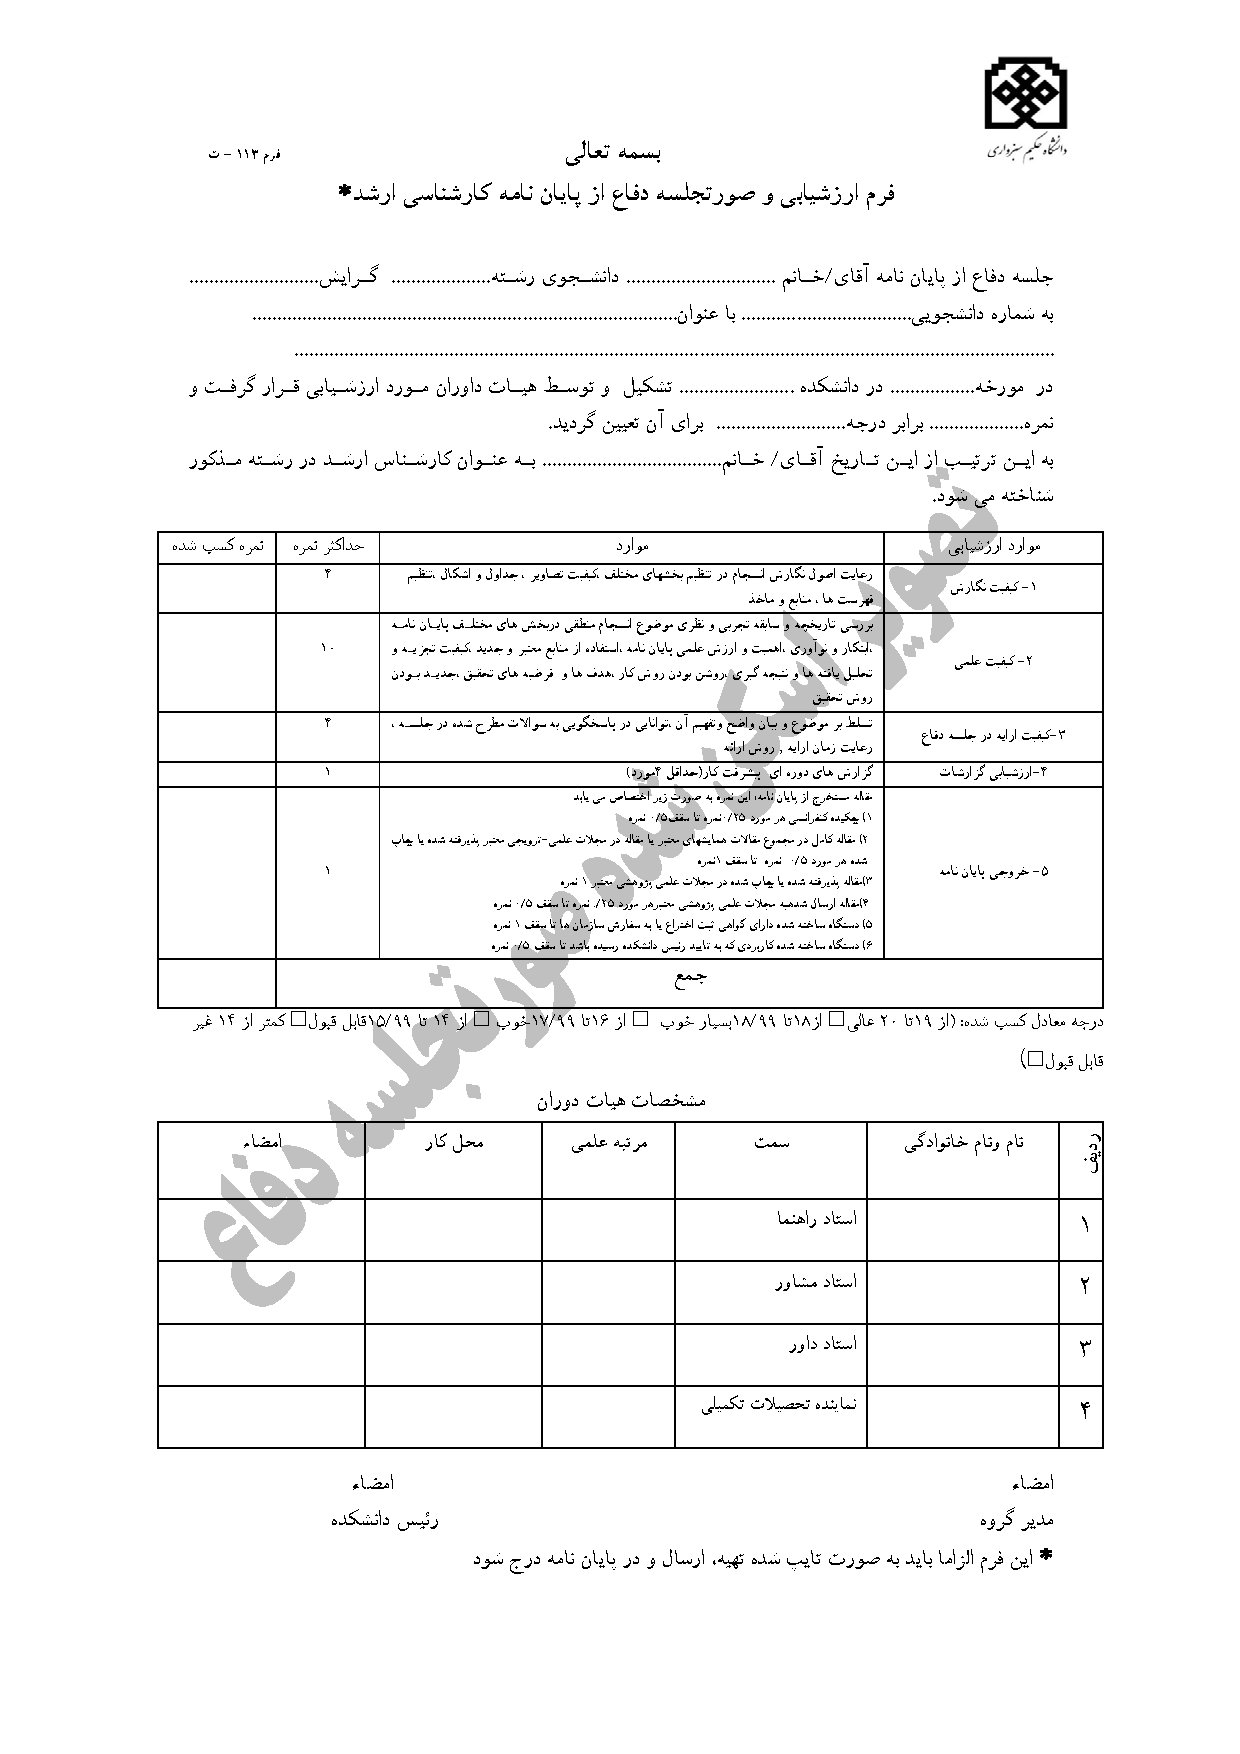
\includepdf{sooratjalaseh.pdf}!
در همان فایل را از حالت توضیح خارج کنید.
\end{enumerate}
دقت داشته باشید که اگر فایل اسکن شده شما، نامی به جز 
\lr{sooratjalaseh}
دارد یا باید نام آنرا به همین عبارت تغییر دهید و یا نام فایل خود را در  دستور فوق قرار دهید.
جدول اطلاعات داوران در فایل
\lr{davaranJadval.tex}
قرار دارد.

\subsection{مراجع}
برای وارد کردن مراجع \پ خود، کافی است فایل 
\lr{MyReferences.bib}
را باز کرده و مراجع خود را مانند مراجع داخل آن، وارد کنید.  سپس از \lr{bibtex} برای تولید مراجع با قالب مناسب استفاده کنید. برای توضیحات بیشتر بخش \ref{Sec:Ref} و پیوست
\eqref{App:App1} را ببینید.


\subsection{واژه‌نامه و نمایه}
برای وارد کردن واژه‌نامه فارسی به انگلیسی و برعکس، چنانچه کاربر مبتدی هستید، بهتر است مانند روش بکار رفته در فایل‌های 
\lr{dicfa2en}
و
\lr{dicen2fa}
عمل کنید. اما چنانچه کاربر پیشرفته هستید، بهتر است از بسته
\lr{glossaries}
استفاده کنید. 
برای وارد کردن نمایه، باید از 
\lr{xindy}
استفاده کنید. 
%زیرا 
%\lr{MakeIndex}
%با حروف «گ»، «چ»، «پ»، «ژ» و «ک» مشکل دارد و ترتیب الفبایی این حروف را رعایت نمی‌کند. همچنین، فاصله بین هر گروه از کلمات در 
%\lr{MakeIndex}،
%به درستی رعایت نمی‌شود که باعث زشت شدن حروف‌چینی این قسمت می‌شود. 
راهنمای چگونگی کار با 
\lr{glossaries} و \lr{xindy} 
را می‌توانید در
 \href{http://wiki.parsilatex.com}{ویکی پارسی‌لاتک} 
 مشاهده فرمایید.

\section{اگر سوالی داشتم، از کی بپرسم؟}
برای پرسیدن سوال های خود موقع حروف‌چینی با زی‌پرشین،  می‌توانید به
 \href{http://qa.parsilatex.com}{سایت پرسش و پاسخ پارسی‌لاتک}%
\LTRfootnote{\url{http://qa.parsilatex.com}}
مراجعه کنید. شما هم می‌توانید روزی به سوال های دیگران در این تالار، جواب بدهید.
بسته ی زی‌پرشین و بسیاری بسته‌های مرتبط با آن مانند \lr{bidi} و \lr{Persian-bib}، مجموعه پارسی‌لاتک، مثالهای مختلف موجود در آن و سایت پارسی‌لاتک همه به صورت داوطلبانه توسط افراد گروه 
\lr{Persian TeX}
و گروه پارسی‌لاتک و بدون هیچ کمک مالی انجام شده‌اند. کار اصلی نوشتن و توسعه زی‌پرشین توسط آقای وفا خلیقی انجام شده است که‌این کار بزرگ را به انجام رساندند.
اگر مایل به کمک به گروه پارسی‌لاتک هستید به سایت گروه پارسی‌لاتک مراجعه فرمایید:
%\begin{center}
 \href{http://www.parsilatex.com}{http://www.parsilatex.com} 
%\end{center}
    
\section{جمع بندی}
در این فصل به بیان مقدمات نحوه استفاده از قالب پایان‌نامه دانشگاه حکیم سبزواری پرداخته شد. گرچه که مطالعه کامل این راهنما مقداری وقت شما را خواهد گرفت، اما مطمئن باشید از اتلاف وقت شما در ادامه کارتان تا حد زیادی جلوگیری خواهد کرد. در نوشتن متن حاضر سعی شده است بیشتر مواردی که عموماً دانشجوان با آن مواجه هستند - و با نگاه ویژه به نیازهای دانشجویان ریاضی - ذکر شود. در ادامه نوشتار نمونه مواردی از درج تصویر، نمودار، کد برنامه، الگوریتم، توضیحات، منابع، فرمول، تعریف، قضیه، مثال و جدول آمده است. توصیه می‌شود یک کپی از کل فایلهای این قالب را جداگانه از نسخه \پ خود نگهداری نمایید تا در صورت نیاز بتوانید مراجعه فرمایید. همچنین توصیه اکید دارم که رفع خطاهایی که احتمالاً با آن مواجه می‌شوید را با آخر موکول نفرمایید و به محض برخورد با خطا، آنرا اشکال‌زدایی نموده و خطا را برطرف فرمایید.

!
و
\verb!% !TEX TS-program = XeLaTeX
% !TeX root=main.tex

\chapter{آشنایی سریع با برخی دستورات لاتک}\label{Chap:chapter2}

در این فصل ویژگی های مهم و پرکاربرد زی‌پرشین و لاتک معرفی می‌شود. برای راهنمایی بیشتر و به کاربردن ویژگی های پیشرفته تر به راهنمای زی‌پرشین و راهنمای لاتک مراجعه کنید. برای آگاهی از دستورات لاتک که‌این خروجی را تولید کرده‌اند فایل \lr{chapter2.tex} را ملاحظه فرمایید.
%\footnote{بیشتر مطالب این بخش از مثال 
%\lr{xepersian\_example.tex}
%گرفته شده‌اند که توسط دوستمان آقای امیرمسعود پورموسی آماده شده بوده است.}

\section{بندها و زیرنویس ها}
هر جایی از نوشتهٔ خود، اگر می خواهید به سر سطر بروید و یک بند تازه را آغاز کنید، باید یک خط را خالی بگذارید.
%\footnote{یعنی دوبار باید کلید \lr{Enter} را بزنید.}
% مانند این:

حالا که یک بند تازه آغاز شده است، یک زیرنویس انگلیسی
\LTRfootnote{English Footnote!}
 هم می نویسیم!
\section{فرمول های ریاضی}\label{formula}

اینجا هم یک فرمول می آوریم که شماره دارد:
\begin{equation}\label{eq:yek}
A=\frac{c}{d}+\frac{q^2}{\sin(\omega t)+\Omega_{12}}
\end{equation}

%\RTLcolumnfootnotes

در لاتک می توان به کمک فرمان 
\lr{\textbackslash label\{\}}
به هر فرمول یک نام نسبت داد. در فرمول بالا نام \lr{eq:yek} را برایش گذاشته‌ایم (پروندهٔ \lr{tex} همراه با این مثال را ببینید). این نام ما را قادر می‌کند که بعداً بتوانیم با فرمان
\lr{\textbackslash ref\{eq:yek\}}
به آن فرمول با شماره ارجاع دهیم. یعنی بنویسیم فرمول \ref{eq:yek}. 
لاتک خودش شمارهٔ این فرمول ها را مدیریت می‌کند. یعنی اگر بعداً فرمولی قبل از این فرمول بنویسیم، خودبه خود شمارهٔ این فرمول و شمارهٔ ارجاع ها به‌این فرمول یکی زیاد می‌شود و لازم نیست نگران شماره گذاری فرمول های خود باشید.

این هم یک فرمول که شماره ندارد:
$$A=|\vec{a}\times \vec{b}| + \sum_{n=0}^\infty C_{ij}$$

این هم عبارتی ریاضی مانند 
$\sqrt{a^2+b^2}$
 که بین متن می آید.

نمایش ارقام در محیط‌های مختلف متفاوت است. به عنوان مثال اگر \lr{0123456789.123} را  در حالت متن و ریاضی فارسی و در حالت معمولی و پررنگ لاتین داشته باشید، خروجی به ترتیب به صورت زیر خواهد بود:
 \begin{LTR}
 \noindent
 0123456789.123\\
 $0123456789.123$\\
 \lr{0123456789.123}\\
\lr{ $\mathbf{0123456789.123}$}\\
\end{LTR}
 ارقام در حالت متن فارسی از قلم فارسی و در متن انگلیسی از قلم انگلیسی گرفته می‌شوند. تغییر نوع و اندازه قلم ارقام در محیط ریاضی با دستور 
\lr{setdigitfont}
در فایل 
\lr{commands}
قابل انجام است. 
   ممکن است خواسته باشید برخی ارقام ریاضی را - مثلاً برای نمایش یک بردار - با حروفی متفاوت نشان دهید، مثل این: 
\begin{LTR}
 \noindent
$\mathsf{0123456789.123}$ 
\end{LTR}


که از دستور 
\verb!\mathsf{0123456789}!
برای نمایش آن استفاده شده است. در این استیل از قلم 
\lr{IRTitr}
در دستور
\verb!\setmathsfdigitfont{IRTitr}!
در فایل 
\lr{commands}
به این منظور استفاده شده است که در صورت نیاز می‌توانید آن‌را تغییر دهید.

\subsection{یک زیربخش}\label{zirbakhsh}

این زیربخش \ref{zirbakhsh} است؛ یعنی یک بخش درون بخش \ref{formula} است.
\subsubsection{یک زیرزیربخش}
این هم یک زیرزیربخش است. در لاتک می‌توانید بخش‌های تودرتو در نوشته تان تعریف کنید تا ساختار منطقی نوشته را به خوبی نشان دهید. می‌توانید به‌این بخش‌ها هم با شماره ارجاع دهید، مثلاً بخش فرمول های ریاضی شماره اش \ref{formula} است.
\section{نوشته‌های فارسی و انگلیسی مخلوط}
نوشتن یک کلمهٔ انگلیسی بین متن فارسی بدیهی است، مانند Example در این جمله.
نوشتن یک عبارت چندکلمه‌ای مانند
 \lr{More than one word} کمی پیچیده تر است.

اگر ناگهان تصمیم بگیرید که یک بند کاملاً انگلیسی را بنویسید، باید:
\begin{latin}
This is an English paragraph from left to right. You can write as much as you want in it.
\end{latin}
\section{افزودن تصویر به نوشته}
پروندهٔ تصویر دلخواه خود را در کنار پروندهٔ \lr{tex} قرار دهید. سپس به روش زیر تصویر را در نوشتهٔ خود بیاورید:
\begin{latin}
\begin{verbatim}
\includegraphics{YourImageFileName}
\end{verbatim}
\end{latin}
به تصویرها هم مانند فرمول ها و بخش‌ها می توان با شماره ارجاع داد. برای جزئیات بیشتر دربارهٔ روش گذاشتن تصویرها در نوشته باید راهنماهای لاتک را بخوانید. نمونه تصاویری در پیوست آمده است که می‌توانید نحوه درج آنها را ملاحظه فرمایید.


\section{محیط های شمارش و نکات}
برای فهرست کردن چندمورد، اگر ترتیب برایمان مهم نباشد:
\begin{itemize}
\item مورد یکم
\item مورد دوم
\item مورد سوم
\end{itemize}
و اگر ترتیب برایمان مهم باشد:
\begin{enumerate}
\item مورد یکم
\item مورد دوم
\item مورد سوم
\end{enumerate}
می توان موردهای تودرتو داشت:
\begin{enumerate}
\item مورد ۱
\item مورد ۲
\begin{enumerate}
\item مورد ۱ از ۲
\item مورد ۲ از ۲
\item مورد ۳ از ۲
\end{enumerate}
\item مورد ۳
\end{enumerate}
شماره گذاری این موردها را هم لاتک انجام می دهد.

\section{تعریف و قضیه}

برای ذکر تعریف، قضیه و مثال مثالهای ذیل را ببینید.

%\textbf{برای ذکر تعریف، قضیه و مثال مثالهای ذیل را ببینید.}
%
%{\iranicfamily برای ذکر تعریف، قضیه و مثال مثالهای ذیل را ببینید.}
%
%\textbf{\emph{ برای ذکر تعریف، قضیه و مثال مثالهای ذیل را ببینید.}}
%
%{\iranicfamily \bf{ برای ذکر تعریف، قضیه و مثال مثالهای ذیل را ببینید.}}

\begin{definition}
مجموعه همه ارزیابی های  (پیوسته)  روی $(X,\tau)$، دامنه توانی احتمالی
\index{دامنه توانی احتمالی}
$ X $
نامیده می‌شود.
\end{definition}
\begin{theorem}[باناخ-آلااغلو]
\index{قضیه باناخ-آلااغلو}
اگر $ V $ یک همسایگی $ 0 $ در فضای برداری 
\index{فضای!برداری}
 توپولوژیکی $ X $ باشد و 
\begin{equation}\label{eq1}
K=\left\lbrace \Lambda \in X^{*}:|\Lambda x|\leqslant 1 ; \ \forall x\in V\right\rbrace,
\end{equation}
آنگاه $ K $،  ضعیف*-فشرده است که در آن، $ X^{*} $ دوگان
\index{فضای!دوگان}
 فضای برداری توپولوژیکی $ X $ است به  طوری که عناصر آن،  تابعی های 
خطی پیوسته
\index{تابعی خطی پیوسته}
 روی $X$ هستند.
\end{theorem}
تساوی \eqref{eq1} یکی از مهم ترین تساوی ها در آنالیز تابعی است که در ادامه، به وفور از آن استفاده می‌شود.
\begin{example}
برای هر فضای مرتب، گردایه 
$$U:=\left\lbrace U\in O: U=\uparrow U\right\rbrace $$
از مجموعه‌های بالایی باز، یک توپولوژی تعریف می‌کند که از توپولوژی اصلی، درشت تر  است.
\end{example}
حال تساوی 
\begin{equation}\label{eq2}
\sum_{n=1}^{+\infty} 3^{n}x+7x=\int_{1}^{n}8nx+\exp{(2nx)}
\end{equation}
را در نظر بگیرید. با مقایسه تساوی \eqref{eq2} با تساوی \eqref{eq1} می توان نتیجه گرفت که ...


\section{چگونگی نوشتن و ارجاع به مراجع}\label{Sec:Ref}

در لاتک به راحتی می توان مراجع خود را نوشت و به آنها ارجاع داد. به عنوان مثال برای معرفی کتاب گنزالس \cite{Gonzalez02book} به عنوان یک مرجع می توان آنرا به صورت زیر معرفی نمود:

\singlespacing
\begin{LTR}
\begin{verbatim}
\bibitem{Gonzalez02book}
Gonzalez, R.C., and Woods, R.E. {\em Digital Image Processing}, 3rd ed..
Prentice-Hall, Inc., Upper Saddle River, NJ, USA, 2006.
\end{verbatim}
\end{LTR}
\doublespacing

در دستورات فوق \lr{Gonzalez02book}  برچسبی است که به‌این مرجع داده شده است و با استفاده از دستور 
\verb!\cite{Gonzalez02book}!
می توان به آن ارجاع داد؛ بدون این که شماره اش را در فهرست مراجع مان بدانیم.

اگر این اولین مرجع ما باشد در قسمت مراجع به صورت زیر خواهد آمد:\\
\begin{latin}

\noindent [1] Gonzalez, Rafael~C. and Woods, Richard~E.  {\em Digital Image Processing}.  Prentice-Hall, 

Inc., Upper Saddle River, NJ, USA, 3rd ed. , 2006.
\end{latin}


این شیوه برای تعداد مراجع کم بد نیست اما اگر فرمت مراجع، ترتیب یا تعداد آنها را خواسته باشید تغییر دهید، به عنوان مثال ابتدا حرف اول نام نویسنده بیاید و سپس نام خانوادگی، باید همه کارها را به صورت دستی انجام دهید.
اگر مایلید کنترل کاملی بر مراجع خود داشته باشید و به راحتی بتوانید قالب مراجع خود را عوض کنید باید از \lr{Bib\TeX} استفاده کنید که درپیوست  \ref{App:App1} به  آن پرداخته خواهد شد.
!
را در فایل 
\lr{main.tex}،
غیرفعال کنید.
برای غیرفعال کردن یک دستور، کافی است در ابتدای آن، یک علامت درصد انگلیسی (\%) بگذارید.
   در غیر این صورت، ابتدا مطالب دو فصل اول  پردازش شده و سپس مطالب فصل ۳ پردازش می‌شود و این کار باعث طولانی شدن زمان اجرا می‌شود. هر زمان که خروجی کل \پ خود را خواستید تمام فصلها را از حالت توضیح خارج کنید.


یک نکته بدیهی که در اینجا وجود دارد، این است که لازم نیست که فصل‌های \پ را به ترتیب تایپ کنید. می‌توانید ابتدا مطالب فصل ۳ را تایپ کنید و سپس مطالب فصل ۱ را تایپ کنید. 
\subsection{فرم ارزشیابی و صورتجلسه دفاع}
فرم ۱۱۳-ت از فرم‌های مربوط به تحصیلات تکمیلی، «فرم ارزشیابی و صورتجلسه دفاع، به همراه مشخصات داوران» است که باید در صفحات آغازین \پ درج شود.
وابسته به اطلاعات \پ این فرم توسط قالب پایان‌نامه آماده می‌شود. اما در نهایت، پس از دفاع باید این فرم اسکن شده و در \پ درج گردد.
برای درج فرم اسکن شده، کافیست:
\begin{enumerate}
\item
دستور 
\verb!\davaranPage!
در اواخر فایل
\lr{faTitle}
را به حالت توضیح درآورید،
\item
  فایل اسکن شده با پسوند 
\lr{PDF}
را در پوشه فایل‌های \پ قرار دهید و
\item
دستور
\verb!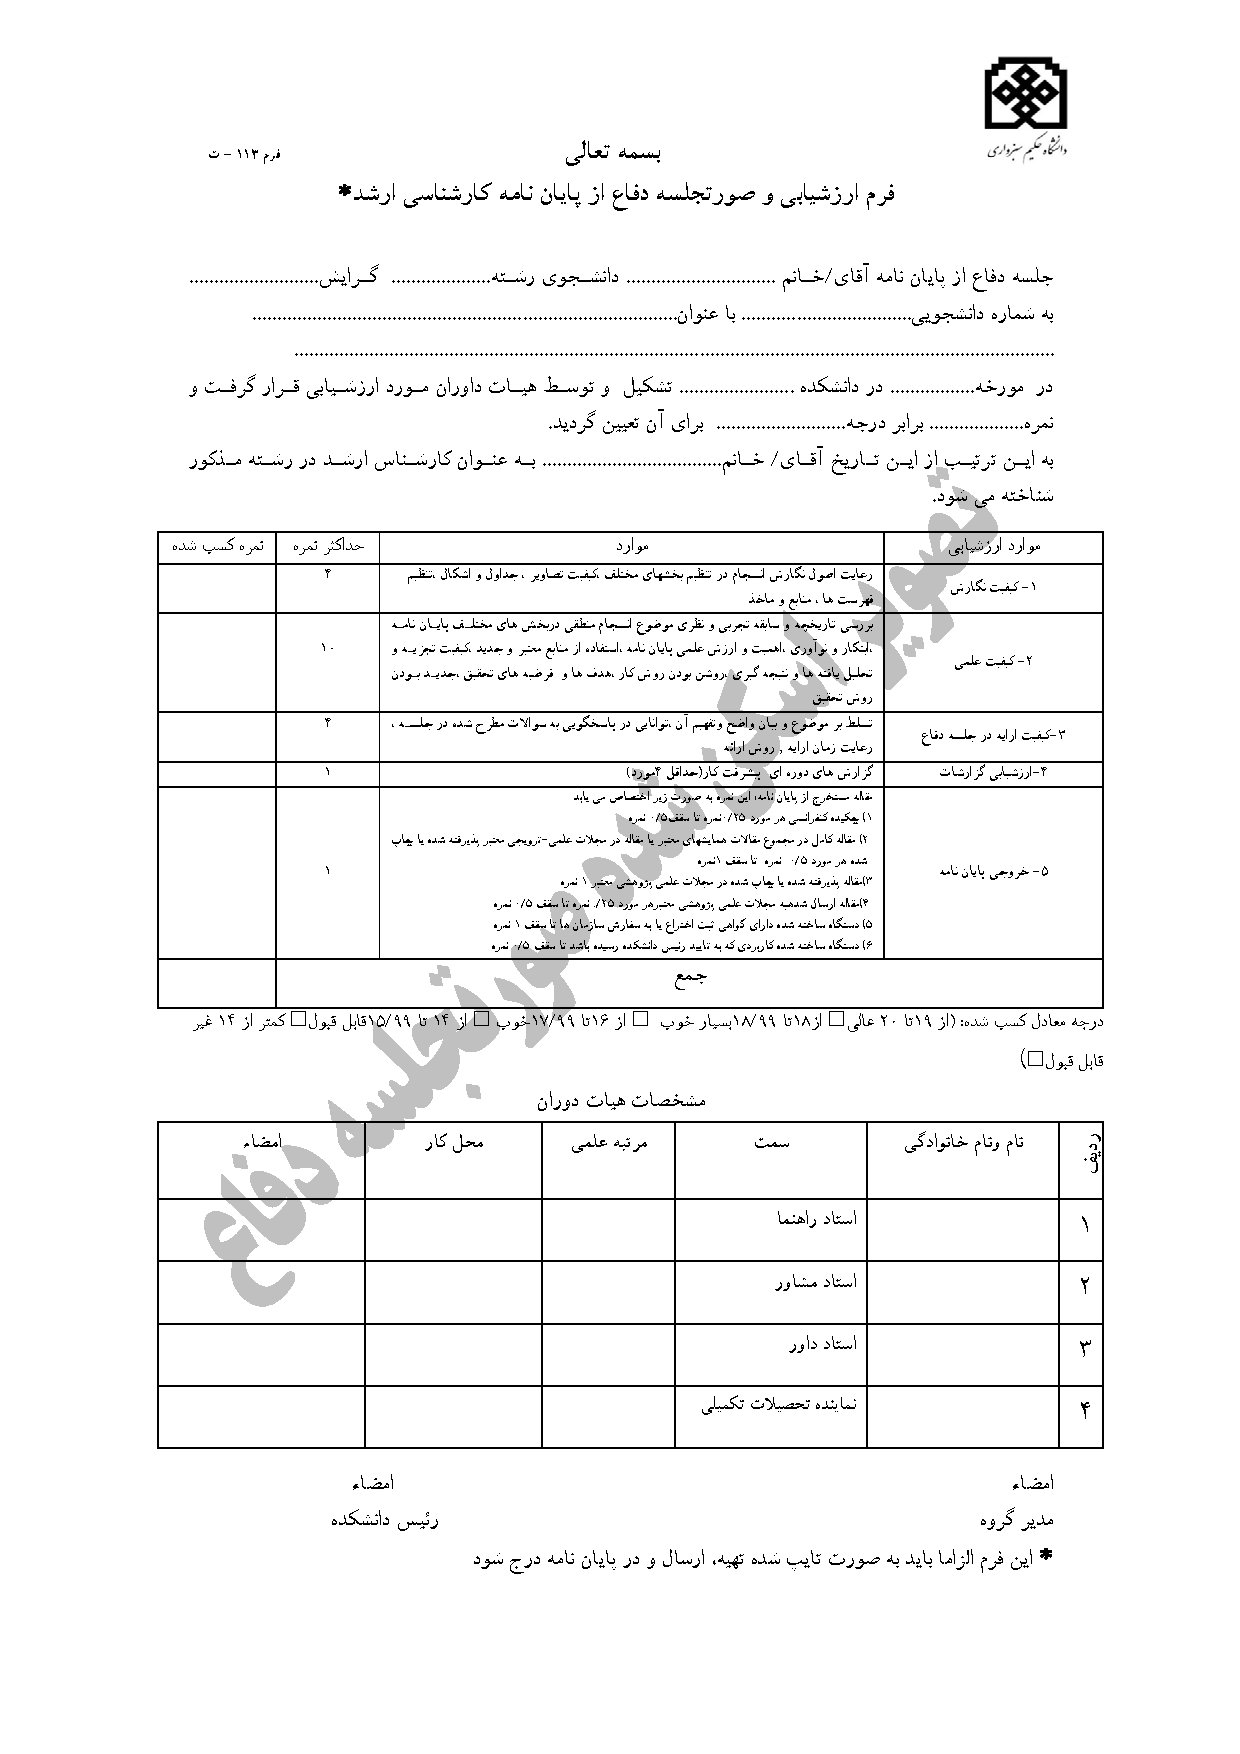
\includepdf{sooratjalaseh.pdf}!
در همان فایل را از حالت توضیح خارج کنید.
\end{enumerate}
دقت داشته باشید که اگر فایل اسکن شده شما، نامی به جز 
\lr{sooratjalaseh}
دارد یا باید نام آنرا به همین عبارت تغییر دهید و یا نام فایل خود را در  دستور فوق قرار دهید.
جدول اطلاعات داوران در فایل
\lr{davaranJadval.tex}
قرار دارد.

\subsection{مراجع}
برای وارد کردن مراجع \پ خود، کافی است فایل 
\lr{MyReferences.bib}
را باز کرده و مراجع خود را مانند مراجع داخل آن، وارد کنید.  سپس از \lr{bibtex} برای تولید مراجع با قالب مناسب استفاده کنید. برای توضیحات بیشتر بخش \ref{Sec:Ref} و پیوست
\eqref{App:App1} را ببینید.


\subsection{واژه‌نامه و نمایه}
برای وارد کردن واژه‌نامه فارسی به انگلیسی و برعکس، چنانچه کاربر مبتدی هستید، بهتر است مانند روش بکار رفته در فایل‌های 
\lr{dicfa2en}
و
\lr{dicen2fa}
عمل کنید. اما چنانچه کاربر پیشرفته هستید، بهتر است از بسته
\lr{glossaries}
استفاده کنید. 
برای وارد کردن نمایه، باید از 
\lr{xindy}
استفاده کنید. 
%زیرا 
%\lr{MakeIndex}
%با حروف «گ»، «چ»، «پ»، «ژ» و «ک» مشکل دارد و ترتیب الفبایی این حروف را رعایت نمی‌کند. همچنین، فاصله بین هر گروه از کلمات در 
%\lr{MakeIndex}،
%به درستی رعایت نمی‌شود که باعث زشت شدن حروف‌چینی این قسمت می‌شود. 
راهنمای چگونگی کار با 
\lr{glossaries} و \lr{xindy} 
را می‌توانید در
 \href{http://wiki.parsilatex.com}{ویکی پارسی‌لاتک} 
 مشاهده فرمایید.

\section{اگر سوالی داشتم، از کی بپرسم؟}
برای پرسیدن سوال های خود موقع حروف‌چینی با زی‌پرشین،  می‌توانید به
 \href{http://qa.parsilatex.com}{سایت پرسش و پاسخ پارسی‌لاتک}%
\LTRfootnote{\url{http://qa.parsilatex.com}}
مراجعه کنید. شما هم می‌توانید روزی به سوال های دیگران در این تالار، جواب بدهید.
بسته ی زی‌پرشین و بسیاری بسته‌های مرتبط با آن مانند \lr{bidi} و \lr{Persian-bib}، مجموعه پارسی‌لاتک، مثالهای مختلف موجود در آن و سایت پارسی‌لاتک همه به صورت داوطلبانه توسط افراد گروه 
\lr{Persian TeX}
و گروه پارسی‌لاتک و بدون هیچ کمک مالی انجام شده‌اند. کار اصلی نوشتن و توسعه زی‌پرشین توسط آقای وفا خلیقی انجام شده است که‌این کار بزرگ را به انجام رساندند.
اگر مایل به کمک به گروه پارسی‌لاتک هستید به سایت گروه پارسی‌لاتک مراجعه فرمایید:
%\begin{center}
 \href{http://www.parsilatex.com}{http://www.parsilatex.com} 
%\end{center}
    
\section{جمع بندی}
در این فصل به بیان مقدمات نحوه استفاده از قالب پایان‌نامه دانشگاه حکیم سبزواری پرداخته شد. گرچه که مطالعه کامل این راهنما مقداری وقت شما را خواهد گرفت، اما مطمئن باشید از اتلاف وقت شما در ادامه کارتان تا حد زیادی جلوگیری خواهد کرد. در نوشتن متن حاضر سعی شده است بیشتر مواردی که عموماً دانشجوان با آن مواجه هستند - و با نگاه ویژه به نیازهای دانشجویان ریاضی - ذکر شود. در ادامه نوشتار نمونه مواردی از درج تصویر، نمودار، کد برنامه، الگوریتم، توضیحات، منابع، فرمول، تعریف، قضیه، مثال و جدول آمده است. توصیه می‌شود یک کپی از کل فایلهای این قالب را جداگانه از نسخه \پ خود نگهداری نمایید تا در صورت نیاز بتوانید مراجعه فرمایید. همچنین توصیه اکید دارم که رفع خطاهایی که احتمالاً با آن مواجه می‌شوید را با آخر موکول نفرمایید و به محض برخورد با خطا، آنرا اشکال‌زدایی نموده و خطا را برطرف فرمایید.

!
و
\verb!% !TEX TS-program = XeLaTeX
% !TeX root=main.tex

\chapter{آشنایی سریع با برخی دستورات لاتک}\label{Chap:chapter2}

در این فصل ویژگی های مهم و پرکاربرد زی‌پرشین و لاتک معرفی می‌شود. برای راهنمایی بیشتر و به کاربردن ویژگی های پیشرفته تر به راهنمای زی‌پرشین و راهنمای لاتک مراجعه کنید. برای آگاهی از دستورات لاتک که‌این خروجی را تولید کرده‌اند فایل \lr{chapter2.tex} را ملاحظه فرمایید.
%\footnote{بیشتر مطالب این بخش از مثال 
%\lr{xepersian\_example.tex}
%گرفته شده‌اند که توسط دوستمان آقای امیرمسعود پورموسی آماده شده بوده است.}

\section{بندها و زیرنویس ها}
هر جایی از نوشتهٔ خود، اگر می خواهید به سر سطر بروید و یک بند تازه را آغاز کنید، باید یک خط را خالی بگذارید.
%\footnote{یعنی دوبار باید کلید \lr{Enter} را بزنید.}
% مانند این:

حالا که یک بند تازه آغاز شده است، یک زیرنویس انگلیسی
\LTRfootnote{English Footnote!}
 هم می نویسیم!
\section{فرمول های ریاضی}\label{formula}

اینجا هم یک فرمول می آوریم که شماره دارد:
\begin{equation}\label{eq:yek}
A=\frac{c}{d}+\frac{q^2}{\sin(\omega t)+\Omega_{12}}
\end{equation}

%\RTLcolumnfootnotes

در لاتک می توان به کمک فرمان 
\lr{\textbackslash label\{\}}
به هر فرمول یک نام نسبت داد. در فرمول بالا نام \lr{eq:yek} را برایش گذاشته‌ایم (پروندهٔ \lr{tex} همراه با این مثال را ببینید). این نام ما را قادر می‌کند که بعداً بتوانیم با فرمان
\lr{\textbackslash ref\{eq:yek\}}
به آن فرمول با شماره ارجاع دهیم. یعنی بنویسیم فرمول \ref{eq:yek}. 
لاتک خودش شمارهٔ این فرمول ها را مدیریت می‌کند. یعنی اگر بعداً فرمولی قبل از این فرمول بنویسیم، خودبه خود شمارهٔ این فرمول و شمارهٔ ارجاع ها به‌این فرمول یکی زیاد می‌شود و لازم نیست نگران شماره گذاری فرمول های خود باشید.

این هم یک فرمول که شماره ندارد:
$$A=|\vec{a}\times \vec{b}| + \sum_{n=0}^\infty C_{ij}$$

این هم عبارتی ریاضی مانند 
$\sqrt{a^2+b^2}$
 که بین متن می آید.

نمایش ارقام در محیط‌های مختلف متفاوت است. به عنوان مثال اگر \lr{0123456789.123} را  در حالت متن و ریاضی فارسی و در حالت معمولی و پررنگ لاتین داشته باشید، خروجی به ترتیب به صورت زیر خواهد بود:
 \begin{LTR}
 \noindent
 0123456789.123\\
 $0123456789.123$\\
 \lr{0123456789.123}\\
\lr{ $\mathbf{0123456789.123}$}\\
\end{LTR}
 ارقام در حالت متن فارسی از قلم فارسی و در متن انگلیسی از قلم انگلیسی گرفته می‌شوند. تغییر نوع و اندازه قلم ارقام در محیط ریاضی با دستور 
\lr{setdigitfont}
در فایل 
\lr{commands}
قابل انجام است. 
   ممکن است خواسته باشید برخی ارقام ریاضی را - مثلاً برای نمایش یک بردار - با حروفی متفاوت نشان دهید، مثل این: 
\begin{LTR}
 \noindent
$\mathsf{0123456789.123}$ 
\end{LTR}


که از دستور 
\verb!\mathsf{0123456789}!
برای نمایش آن استفاده شده است. در این استیل از قلم 
\lr{IRTitr}
در دستور
\verb!\setmathsfdigitfont{IRTitr}!
در فایل 
\lr{commands}
به این منظور استفاده شده است که در صورت نیاز می‌توانید آن‌را تغییر دهید.

\subsection{یک زیربخش}\label{zirbakhsh}

این زیربخش \ref{zirbakhsh} است؛ یعنی یک بخش درون بخش \ref{formula} است.
\subsubsection{یک زیرزیربخش}
این هم یک زیرزیربخش است. در لاتک می‌توانید بخش‌های تودرتو در نوشته تان تعریف کنید تا ساختار منطقی نوشته را به خوبی نشان دهید. می‌توانید به‌این بخش‌ها هم با شماره ارجاع دهید، مثلاً بخش فرمول های ریاضی شماره اش \ref{formula} است.
\section{نوشته‌های فارسی و انگلیسی مخلوط}
نوشتن یک کلمهٔ انگلیسی بین متن فارسی بدیهی است، مانند Example در این جمله.
نوشتن یک عبارت چندکلمه‌ای مانند
 \lr{More than one word} کمی پیچیده تر است.

اگر ناگهان تصمیم بگیرید که یک بند کاملاً انگلیسی را بنویسید، باید:
\begin{latin}
This is an English paragraph from left to right. You can write as much as you want in it.
\end{latin}
\section{افزودن تصویر به نوشته}
پروندهٔ تصویر دلخواه خود را در کنار پروندهٔ \lr{tex} قرار دهید. سپس به روش زیر تصویر را در نوشتهٔ خود بیاورید:
\begin{latin}
\begin{verbatim}
\includegraphics{YourImageFileName}
\end{verbatim}
\end{latin}
به تصویرها هم مانند فرمول ها و بخش‌ها می توان با شماره ارجاع داد. برای جزئیات بیشتر دربارهٔ روش گذاشتن تصویرها در نوشته باید راهنماهای لاتک را بخوانید. نمونه تصاویری در پیوست آمده است که می‌توانید نحوه درج آنها را ملاحظه فرمایید.


\section{محیط های شمارش و نکات}
برای فهرست کردن چندمورد، اگر ترتیب برایمان مهم نباشد:
\begin{itemize}
\item مورد یکم
\item مورد دوم
\item مورد سوم
\end{itemize}
و اگر ترتیب برایمان مهم باشد:
\begin{enumerate}
\item مورد یکم
\item مورد دوم
\item مورد سوم
\end{enumerate}
می توان موردهای تودرتو داشت:
\begin{enumerate}
\item مورد ۱
\item مورد ۲
\begin{enumerate}
\item مورد ۱ از ۲
\item مورد ۲ از ۲
\item مورد ۳ از ۲
\end{enumerate}
\item مورد ۳
\end{enumerate}
شماره گذاری این موردها را هم لاتک انجام می دهد.

\section{تعریف و قضیه}

برای ذکر تعریف، قضیه و مثال مثالهای ذیل را ببینید.

%\textbf{برای ذکر تعریف، قضیه و مثال مثالهای ذیل را ببینید.}
%
%{\iranicfamily برای ذکر تعریف، قضیه و مثال مثالهای ذیل را ببینید.}
%
%\textbf{\emph{ برای ذکر تعریف، قضیه و مثال مثالهای ذیل را ببینید.}}
%
%{\iranicfamily \bf{ برای ذکر تعریف، قضیه و مثال مثالهای ذیل را ببینید.}}

\begin{definition}
مجموعه همه ارزیابی های  (پیوسته)  روی $(X,\tau)$، دامنه توانی احتمالی
\index{دامنه توانی احتمالی}
$ X $
نامیده می‌شود.
\end{definition}
\begin{theorem}[باناخ-آلااغلو]
\index{قضیه باناخ-آلااغلو}
اگر $ V $ یک همسایگی $ 0 $ در فضای برداری 
\index{فضای!برداری}
 توپولوژیکی $ X $ باشد و 
\begin{equation}\label{eq1}
K=\left\lbrace \Lambda \in X^{*}:|\Lambda x|\leqslant 1 ; \ \forall x\in V\right\rbrace,
\end{equation}
آنگاه $ K $،  ضعیف*-فشرده است که در آن، $ X^{*} $ دوگان
\index{فضای!دوگان}
 فضای برداری توپولوژیکی $ X $ است به  طوری که عناصر آن،  تابعی های 
خطی پیوسته
\index{تابعی خطی پیوسته}
 روی $X$ هستند.
\end{theorem}
تساوی \eqref{eq1} یکی از مهم ترین تساوی ها در آنالیز تابعی است که در ادامه، به وفور از آن استفاده می‌شود.
\begin{example}
برای هر فضای مرتب، گردایه 
$$U:=\left\lbrace U\in O: U=\uparrow U\right\rbrace $$
از مجموعه‌های بالایی باز، یک توپولوژی تعریف می‌کند که از توپولوژی اصلی، درشت تر  است.
\end{example}
حال تساوی 
\begin{equation}\label{eq2}
\sum_{n=1}^{+\infty} 3^{n}x+7x=\int_{1}^{n}8nx+\exp{(2nx)}
\end{equation}
را در نظر بگیرید. با مقایسه تساوی \eqref{eq2} با تساوی \eqref{eq1} می توان نتیجه گرفت که ...


\section{چگونگی نوشتن و ارجاع به مراجع}\label{Sec:Ref}

در لاتک به راحتی می توان مراجع خود را نوشت و به آنها ارجاع داد. به عنوان مثال برای معرفی کتاب گنزالس \cite{Gonzalez02book} به عنوان یک مرجع می توان آنرا به صورت زیر معرفی نمود:

\singlespacing
\begin{LTR}
\begin{verbatim}
\bibitem{Gonzalez02book}
Gonzalez, R.C., and Woods, R.E. {\em Digital Image Processing}, 3rd ed..
Prentice-Hall, Inc., Upper Saddle River, NJ, USA, 2006.
\end{verbatim}
\end{LTR}
\doublespacing

در دستورات فوق \lr{Gonzalez02book}  برچسبی است که به‌این مرجع داده شده است و با استفاده از دستور 
\verb!\cite{Gonzalez02book}!
می توان به آن ارجاع داد؛ بدون این که شماره اش را در فهرست مراجع مان بدانیم.

اگر این اولین مرجع ما باشد در قسمت مراجع به صورت زیر خواهد آمد:\\
\begin{latin}

\noindent [1] Gonzalez, Rafael~C. and Woods, Richard~E.  {\em Digital Image Processing}.  Prentice-Hall, 

Inc., Upper Saddle River, NJ, USA, 3rd ed. , 2006.
\end{latin}


این شیوه برای تعداد مراجع کم بد نیست اما اگر فرمت مراجع، ترتیب یا تعداد آنها را خواسته باشید تغییر دهید، به عنوان مثال ابتدا حرف اول نام نویسنده بیاید و سپس نام خانوادگی، باید همه کارها را به صورت دستی انجام دهید.
اگر مایلید کنترل کاملی بر مراجع خود داشته باشید و به راحتی بتوانید قالب مراجع خود را عوض کنید باید از \lr{Bib\TeX} استفاده کنید که درپیوست  \ref{App:App1} به  آن پرداخته خواهد شد.
!
را در فایل 
\lr{main.tex}،
غیرفعال کنید.
برای غیرفعال کردن یک دستور، کافی است در ابتدای آن، یک علامت درصد انگلیسی (\%) بگذارید.
   در غیر این صورت، ابتدا مطالب دو فصل اول  پردازش شده و سپس مطالب فصل ۳ پردازش می‌شود و این کار باعث طولانی شدن زمان اجرا می‌شود. هر زمان که خروجی کل \پ خود را خواستید تمام فصلها را از حالت توضیح خارج کنید.


یک نکته بدیهی که در اینجا وجود دارد، این است که لازم نیست که فصل‌های \پ را به ترتیب تایپ کنید. می‌توانید ابتدا مطالب فصل ۳ را تایپ کنید و سپس مطالب فصل ۱ را تایپ کنید. 
\subsection{فرم ارزشیابی و صورتجلسه دفاع}
فرم ۱۱۳-ت از فرم‌های مربوط به تحصیلات تکمیلی، «فرم ارزشیابی و صورتجلسه دفاع، به همراه مشخصات داوران» است که باید در صفحات آغازین \پ درج شود.
وابسته به اطلاعات \پ این فرم توسط قالب پایان‌نامه آماده می‌شود. اما در نهایت، پس از دفاع باید این فرم اسکن شده و در \پ درج گردد.
برای درج فرم اسکن شده، کافیست:
\begin{enumerate}
\item
دستور 
\verb!\davaranPage!
در اواخر فایل
\lr{faTitle}
را به حالت توضیح درآورید،
\item
  فایل اسکن شده با پسوند 
\lr{PDF}
را در پوشه فایل‌های \پ قرار دهید و
\item
دستور
\verb!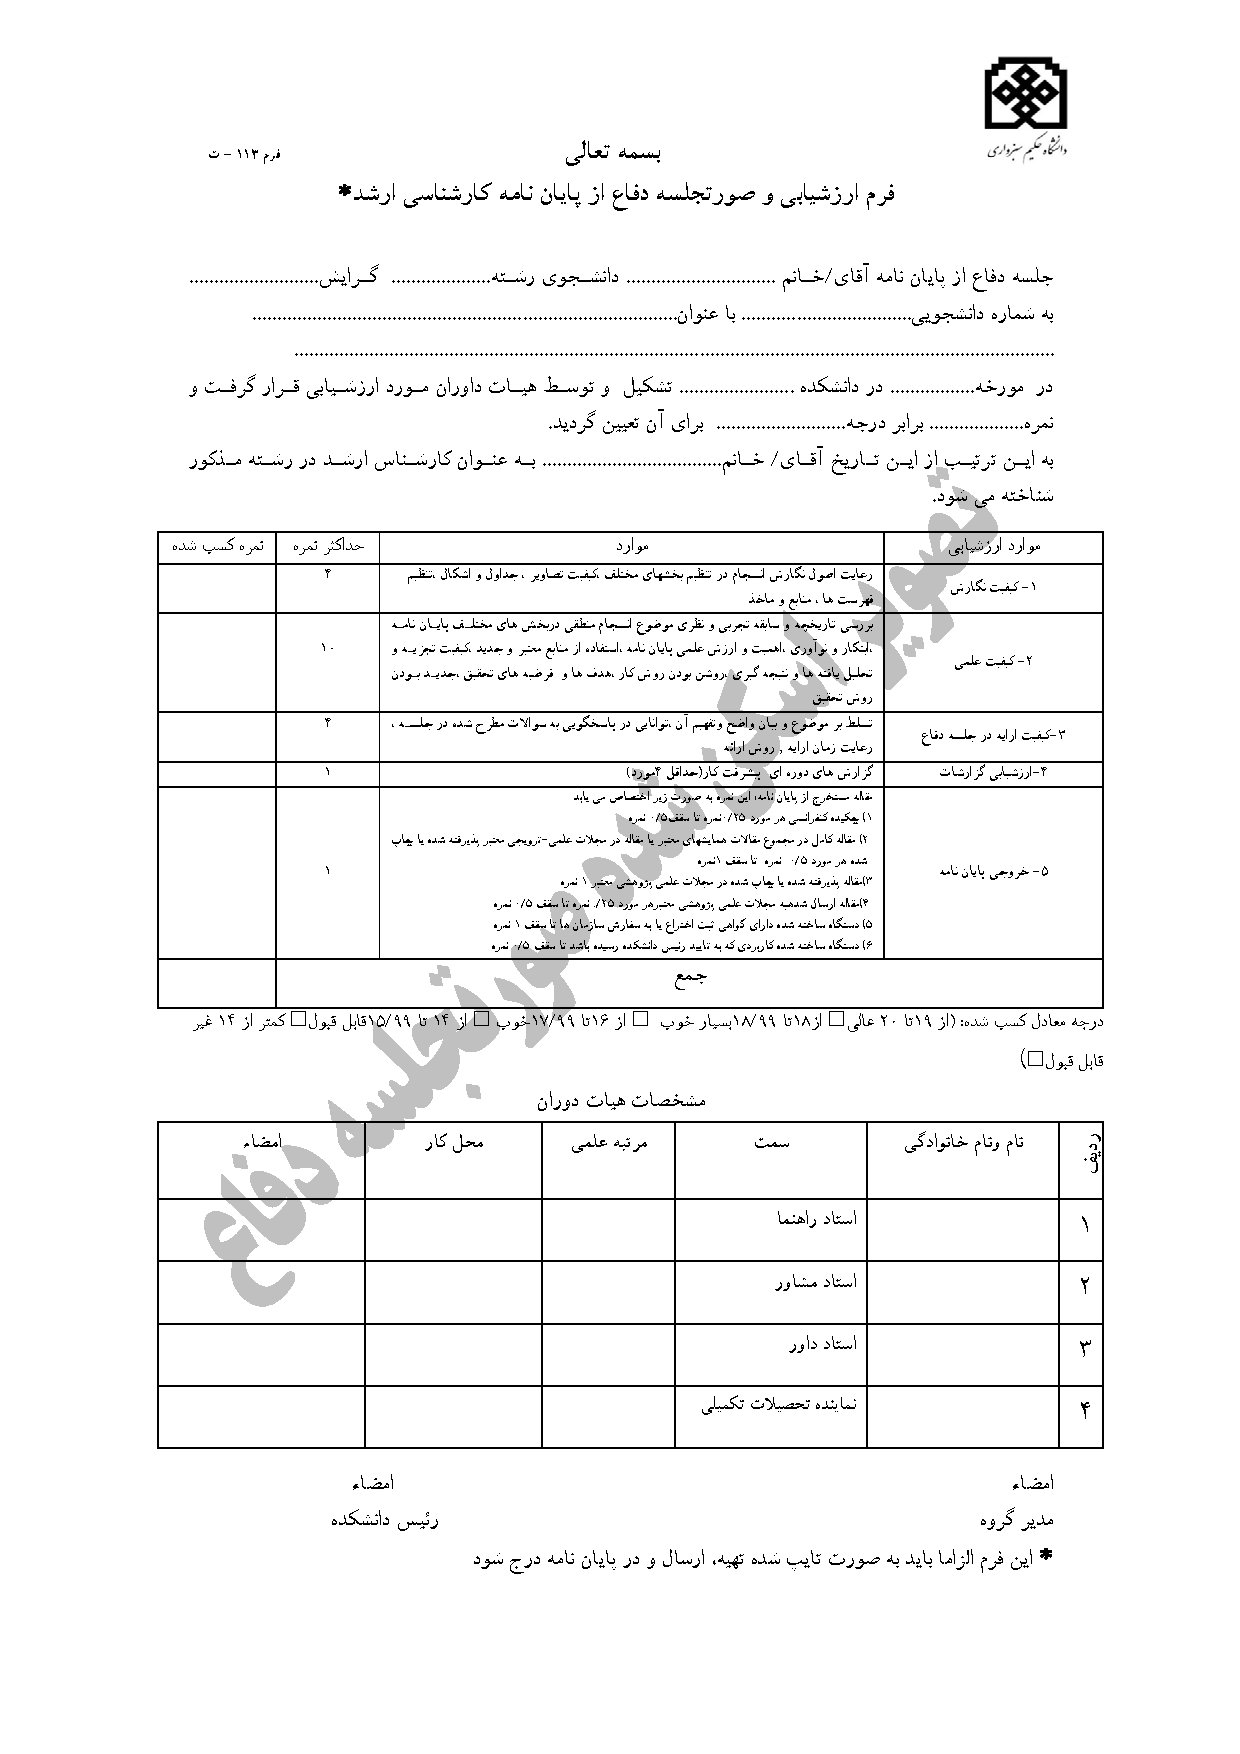
\includepdf{sooratjalaseh.pdf}!
در همان فایل را از حالت توضیح خارج کنید.
\end{enumerate}
دقت داشته باشید که اگر فایل اسکن شده شما، نامی به جز 
\lr{sooratjalaseh}
دارد یا باید نام آنرا به همین عبارت تغییر دهید و یا نام فایل خود را در  دستور فوق قرار دهید.
جدول اطلاعات داوران در فایل
\lr{davaranJadval.tex}
قرار دارد.

\subsection{مراجع}
برای وارد کردن مراجع \پ خود، کافی است فایل 
\lr{MyReferences.bib}
را باز کرده و مراجع خود را مانند مراجع داخل آن، وارد کنید.  سپس از \lr{bibtex} برای تولید مراجع با قالب مناسب استفاده کنید. برای توضیحات بیشتر بخش \ref{Sec:Ref} و پیوست
\eqref{App:App1} را ببینید.


\subsection{واژه‌نامه و نمایه}
برای وارد کردن واژه‌نامه فارسی به انگلیسی و برعکس، چنانچه کاربر مبتدی هستید، بهتر است مانند روش بکار رفته در فایل‌های 
\lr{dicfa2en}
و
\lr{dicen2fa}
عمل کنید. اما چنانچه کاربر پیشرفته هستید، بهتر است از بسته
\lr{glossaries}
استفاده کنید. 
برای وارد کردن نمایه، باید از 
\lr{xindy}
استفاده کنید. 
%زیرا 
%\lr{MakeIndex}
%با حروف «گ»، «چ»، «پ»، «ژ» و «ک» مشکل دارد و ترتیب الفبایی این حروف را رعایت نمی‌کند. همچنین، فاصله بین هر گروه از کلمات در 
%\lr{MakeIndex}،
%به درستی رعایت نمی‌شود که باعث زشت شدن حروف‌چینی این قسمت می‌شود. 
راهنمای چگونگی کار با 
\lr{glossaries} و \lr{xindy} 
را می‌توانید در
 \href{http://wiki.parsilatex.com}{ویکی پارسی‌لاتک} 
 مشاهده فرمایید.

\section{اگر سوالی داشتم، از کی بپرسم؟}
برای پرسیدن سوال های خود موقع حروف‌چینی با زی‌پرشین،  می‌توانید به
 \href{http://qa.parsilatex.com}{سایت پرسش و پاسخ پارسی‌لاتک}%
\LTRfootnote{\url{http://qa.parsilatex.com}}
مراجعه کنید. شما هم می‌توانید روزی به سوال های دیگران در این تالار، جواب بدهید.
بسته ی زی‌پرشین و بسیاری بسته‌های مرتبط با آن مانند \lr{bidi} و \lr{Persian-bib}، مجموعه پارسی‌لاتک، مثالهای مختلف موجود در آن و سایت پارسی‌لاتک همه به صورت داوطلبانه توسط افراد گروه 
\lr{Persian TeX}
و گروه پارسی‌لاتک و بدون هیچ کمک مالی انجام شده‌اند. کار اصلی نوشتن و توسعه زی‌پرشین توسط آقای وفا خلیقی انجام شده است که‌این کار بزرگ را به انجام رساندند.
اگر مایل به کمک به گروه پارسی‌لاتک هستید به سایت گروه پارسی‌لاتک مراجعه فرمایید:
%\begin{center}
 \href{http://www.parsilatex.com}{http://www.parsilatex.com} 
%\end{center}
    
\section{جمع بندی}
در این فصل به بیان مقدمات نحوه استفاده از قالب پایان‌نامه دانشگاه حکیم سبزواری پرداخته شد. گرچه که مطالعه کامل این راهنما مقداری وقت شما را خواهد گرفت، اما مطمئن باشید از اتلاف وقت شما در ادامه کارتان تا حد زیادی جلوگیری خواهد کرد. در نوشتن متن حاضر سعی شده است بیشتر مواردی که عموماً دانشجوان با آن مواجه هستند - و با نگاه ویژه به نیازهای دانشجویان ریاضی - ذکر شود. در ادامه نوشتار نمونه مواردی از درج تصویر، نمودار، کد برنامه، الگوریتم، توضیحات، منابع، فرمول، تعریف، قضیه، مثال و جدول آمده است. توصیه می‌شود یک کپی از کل فایلهای این قالب را جداگانه از نسخه \پ خود نگهداری نمایید تا در صورت نیاز بتوانید مراجعه فرمایید. همچنین توصیه اکید دارم که رفع خطاهایی که احتمالاً با آن مواجه می‌شوید را با آخر موکول نفرمایید و به محض برخورد با خطا، آنرا اشکال‌زدایی نموده و خطا را برطرف فرمایید.

!
و
\verb!% !TEX TS-program = XeLaTeX
% !TeX root=main.tex

\chapter{آشنایی سریع با برخی دستورات لاتک}\label{Chap:chapter2}

در این فصل ویژگی های مهم و پرکاربرد زی‌پرشین و لاتک معرفی می‌شود. برای راهنمایی بیشتر و به کاربردن ویژگی های پیشرفته تر به راهنمای زی‌پرشین و راهنمای لاتک مراجعه کنید. برای آگاهی از دستورات لاتک که‌این خروجی را تولید کرده‌اند فایل \lr{chapter2.tex} را ملاحظه فرمایید.
%\footnote{بیشتر مطالب این بخش از مثال 
%\lr{xepersian\_example.tex}
%گرفته شده‌اند که توسط دوستمان آقای امیرمسعود پورموسی آماده شده بوده است.}

\section{بندها و زیرنویس ها}
هر جایی از نوشتهٔ خود، اگر می خواهید به سر سطر بروید و یک بند تازه را آغاز کنید، باید یک خط را خالی بگذارید.
%\footnote{یعنی دوبار باید کلید \lr{Enter} را بزنید.}
% مانند این:

حالا که یک بند تازه آغاز شده است، یک زیرنویس انگلیسی
\LTRfootnote{English Footnote!}
 هم می نویسیم!
\section{فرمول های ریاضی}\label{formula}

اینجا هم یک فرمول می آوریم که شماره دارد:
\begin{equation}\label{eq:yek}
A=\frac{c}{d}+\frac{q^2}{\sin(\omega t)+\Omega_{12}}
\end{equation}

%\RTLcolumnfootnotes

در لاتک می توان به کمک فرمان 
\lr{\textbackslash label\{\}}
به هر فرمول یک نام نسبت داد. در فرمول بالا نام \lr{eq:yek} را برایش گذاشته‌ایم (پروندهٔ \lr{tex} همراه با این مثال را ببینید). این نام ما را قادر می‌کند که بعداً بتوانیم با فرمان
\lr{\textbackslash ref\{eq:yek\}}
به آن فرمول با شماره ارجاع دهیم. یعنی بنویسیم فرمول \ref{eq:yek}. 
لاتک خودش شمارهٔ این فرمول ها را مدیریت می‌کند. یعنی اگر بعداً فرمولی قبل از این فرمول بنویسیم، خودبه خود شمارهٔ این فرمول و شمارهٔ ارجاع ها به‌این فرمول یکی زیاد می‌شود و لازم نیست نگران شماره گذاری فرمول های خود باشید.

این هم یک فرمول که شماره ندارد:
$$A=|\vec{a}\times \vec{b}| + \sum_{n=0}^\infty C_{ij}$$

این هم عبارتی ریاضی مانند 
$\sqrt{a^2+b^2}$
 که بین متن می آید.

نمایش ارقام در محیط‌های مختلف متفاوت است. به عنوان مثال اگر \lr{0123456789.123} را  در حالت متن و ریاضی فارسی و در حالت معمولی و پررنگ لاتین داشته باشید، خروجی به ترتیب به صورت زیر خواهد بود:
 \begin{LTR}
 \noindent
 0123456789.123\\
 $0123456789.123$\\
 \lr{0123456789.123}\\
\lr{ $\mathbf{0123456789.123}$}\\
\end{LTR}
 ارقام در حالت متن فارسی از قلم فارسی و در متن انگلیسی از قلم انگلیسی گرفته می‌شوند. تغییر نوع و اندازه قلم ارقام در محیط ریاضی با دستور 
\lr{setdigitfont}
در فایل 
\lr{commands}
قابل انجام است. 
   ممکن است خواسته باشید برخی ارقام ریاضی را - مثلاً برای نمایش یک بردار - با حروفی متفاوت نشان دهید، مثل این: 
\begin{LTR}
 \noindent
$\mathsf{0123456789.123}$ 
\end{LTR}


که از دستور 
\verb!\mathsf{0123456789}!
برای نمایش آن استفاده شده است. در این استیل از قلم 
\lr{IRTitr}
در دستور
\verb!\setmathsfdigitfont{IRTitr}!
در فایل 
\lr{commands}
به این منظور استفاده شده است که در صورت نیاز می‌توانید آن‌را تغییر دهید.

\subsection{یک زیربخش}\label{zirbakhsh}

این زیربخش \ref{zirbakhsh} است؛ یعنی یک بخش درون بخش \ref{formula} است.
\subsubsection{یک زیرزیربخش}
این هم یک زیرزیربخش است. در لاتک می‌توانید بخش‌های تودرتو در نوشته تان تعریف کنید تا ساختار منطقی نوشته را به خوبی نشان دهید. می‌توانید به‌این بخش‌ها هم با شماره ارجاع دهید، مثلاً بخش فرمول های ریاضی شماره اش \ref{formula} است.
\section{نوشته‌های فارسی و انگلیسی مخلوط}
نوشتن یک کلمهٔ انگلیسی بین متن فارسی بدیهی است، مانند Example در این جمله.
نوشتن یک عبارت چندکلمه‌ای مانند
 \lr{More than one word} کمی پیچیده تر است.

اگر ناگهان تصمیم بگیرید که یک بند کاملاً انگلیسی را بنویسید، باید:
\begin{latin}
This is an English paragraph from left to right. You can write as much as you want in it.
\end{latin}
\section{افزودن تصویر به نوشته}
پروندهٔ تصویر دلخواه خود را در کنار پروندهٔ \lr{tex} قرار دهید. سپس به روش زیر تصویر را در نوشتهٔ خود بیاورید:
\begin{latin}
\begin{verbatim}
\includegraphics{YourImageFileName}
\end{verbatim}
\end{latin}
به تصویرها هم مانند فرمول ها و بخش‌ها می توان با شماره ارجاع داد. برای جزئیات بیشتر دربارهٔ روش گذاشتن تصویرها در نوشته باید راهنماهای لاتک را بخوانید. نمونه تصاویری در پیوست آمده است که می‌توانید نحوه درج آنها را ملاحظه فرمایید.


\section{محیط های شمارش و نکات}
برای فهرست کردن چندمورد، اگر ترتیب برایمان مهم نباشد:
\begin{itemize}
\item مورد یکم
\item مورد دوم
\item مورد سوم
\end{itemize}
و اگر ترتیب برایمان مهم باشد:
\begin{enumerate}
\item مورد یکم
\item مورد دوم
\item مورد سوم
\end{enumerate}
می توان موردهای تودرتو داشت:
\begin{enumerate}
\item مورد ۱
\item مورد ۲
\begin{enumerate}
\item مورد ۱ از ۲
\item مورد ۲ از ۲
\item مورد ۳ از ۲
\end{enumerate}
\item مورد ۳
\end{enumerate}
شماره گذاری این موردها را هم لاتک انجام می دهد.

\section{تعریف و قضیه}

برای ذکر تعریف، قضیه و مثال مثالهای ذیل را ببینید.

%\textbf{برای ذکر تعریف، قضیه و مثال مثالهای ذیل را ببینید.}
%
%{\iranicfamily برای ذکر تعریف، قضیه و مثال مثالهای ذیل را ببینید.}
%
%\textbf{\emph{ برای ذکر تعریف، قضیه و مثال مثالهای ذیل را ببینید.}}
%
%{\iranicfamily \bf{ برای ذکر تعریف، قضیه و مثال مثالهای ذیل را ببینید.}}

\begin{definition}
مجموعه همه ارزیابی های  (پیوسته)  روی $(X,\tau)$، دامنه توانی احتمالی
\index{دامنه توانی احتمالی}
$ X $
نامیده می‌شود.
\end{definition}
\begin{theorem}[باناخ-آلااغلو]
\index{قضیه باناخ-آلااغلو}
اگر $ V $ یک همسایگی $ 0 $ در فضای برداری 
\index{فضای!برداری}
 توپولوژیکی $ X $ باشد و 
\begin{equation}\label{eq1}
K=\left\lbrace \Lambda \in X^{*}:|\Lambda x|\leqslant 1 ; \ \forall x\in V\right\rbrace,
\end{equation}
آنگاه $ K $،  ضعیف*-فشرده است که در آن، $ X^{*} $ دوگان
\index{فضای!دوگان}
 فضای برداری توپولوژیکی $ X $ است به  طوری که عناصر آن،  تابعی های 
خطی پیوسته
\index{تابعی خطی پیوسته}
 روی $X$ هستند.
\end{theorem}
تساوی \eqref{eq1} یکی از مهم ترین تساوی ها در آنالیز تابعی است که در ادامه، به وفور از آن استفاده می‌شود.
\begin{example}
برای هر فضای مرتب، گردایه 
$$U:=\left\lbrace U\in O: U=\uparrow U\right\rbrace $$
از مجموعه‌های بالایی باز، یک توپولوژی تعریف می‌کند که از توپولوژی اصلی، درشت تر  است.
\end{example}
حال تساوی 
\begin{equation}\label{eq2}
\sum_{n=1}^{+\infty} 3^{n}x+7x=\int_{1}^{n}8nx+\exp{(2nx)}
\end{equation}
را در نظر بگیرید. با مقایسه تساوی \eqref{eq2} با تساوی \eqref{eq1} می توان نتیجه گرفت که ...


\section{چگونگی نوشتن و ارجاع به مراجع}\label{Sec:Ref}

در لاتک به راحتی می توان مراجع خود را نوشت و به آنها ارجاع داد. به عنوان مثال برای معرفی کتاب گنزالس \cite{Gonzalez02book} به عنوان یک مرجع می توان آنرا به صورت زیر معرفی نمود:

\singlespacing
\begin{LTR}
\begin{verbatim}
\bibitem{Gonzalez02book}
Gonzalez, R.C., and Woods, R.E. {\em Digital Image Processing}, 3rd ed..
Prentice-Hall, Inc., Upper Saddle River, NJ, USA, 2006.
\end{verbatim}
\end{LTR}
\doublespacing

در دستورات فوق \lr{Gonzalez02book}  برچسبی است که به‌این مرجع داده شده است و با استفاده از دستور 
\verb!\cite{Gonzalez02book}!
می توان به آن ارجاع داد؛ بدون این که شماره اش را در فهرست مراجع مان بدانیم.

اگر این اولین مرجع ما باشد در قسمت مراجع به صورت زیر خواهد آمد:\\
\begin{latin}

\noindent [1] Gonzalez, Rafael~C. and Woods, Richard~E.  {\em Digital Image Processing}.  Prentice-Hall, 

Inc., Upper Saddle River, NJ, USA, 3rd ed. , 2006.
\end{latin}


این شیوه برای تعداد مراجع کم بد نیست اما اگر فرمت مراجع، ترتیب یا تعداد آنها را خواسته باشید تغییر دهید، به عنوان مثال ابتدا حرف اول نام نویسنده بیاید و سپس نام خانوادگی، باید همه کارها را به صورت دستی انجام دهید.
اگر مایلید کنترل کاملی بر مراجع خود داشته باشید و به راحتی بتوانید قالب مراجع خود را عوض کنید باید از \lr{Bib\TeX} استفاده کنید که درپیوست  \ref{App:App1} به  آن پرداخته خواهد شد.
!
را در فایل 
\lr{main.tex}،
غیرفعال کنید.
برای غیرفعال کردن یک دستور، کافی است در ابتدای آن، یک علامت درصد انگلیسی (\%) بگذارید.
   در غیر این صورت، ابتدا مطالب دو فصل اول  پردازش شده و سپس مطالب فصل ۳ پردازش می‌شود و این کار باعث طولانی شدن زمان اجرا می‌شود. هر زمان که خروجی کل \پ خود را خواستید تمام فصلها را از حالت توضیح خارج کنید.


یک نکته بدیهی که در اینجا وجود دارد، این است که لازم نیست که فصل‌های \پ را به ترتیب تایپ کنید. می‌توانید ابتدا مطالب فصل ۳ را تایپ کنید و سپس مطالب فصل ۱ را تایپ کنید. 
\subsection{فرم ارزشیابی و صورتجلسه دفاع}
فرم ۱۱۳-ت از فرم‌های مربوط به تحصیلات تکمیلی، «فرم ارزشیابی و صورتجلسه دفاع، به همراه مشخصات داوران» است که باید در صفحات آغازین \پ درج شود.
وابسته به اطلاعات \پ این فرم توسط قالب پایان‌نامه آماده می‌شود. اما در نهایت، پس از دفاع باید این فرم اسکن شده و در \پ درج گردد.
برای درج فرم اسکن شده، کافیست:
\begin{enumerate}
\item
دستور 
\verb!\davaranPage!
در اواخر فایل
\lr{faTitle}
را به حالت توضیح درآورید،
\item
  فایل اسکن شده با پسوند 
\lr{PDF}
را در پوشه فایل‌های \پ قرار دهید و
\item
دستور
\verb!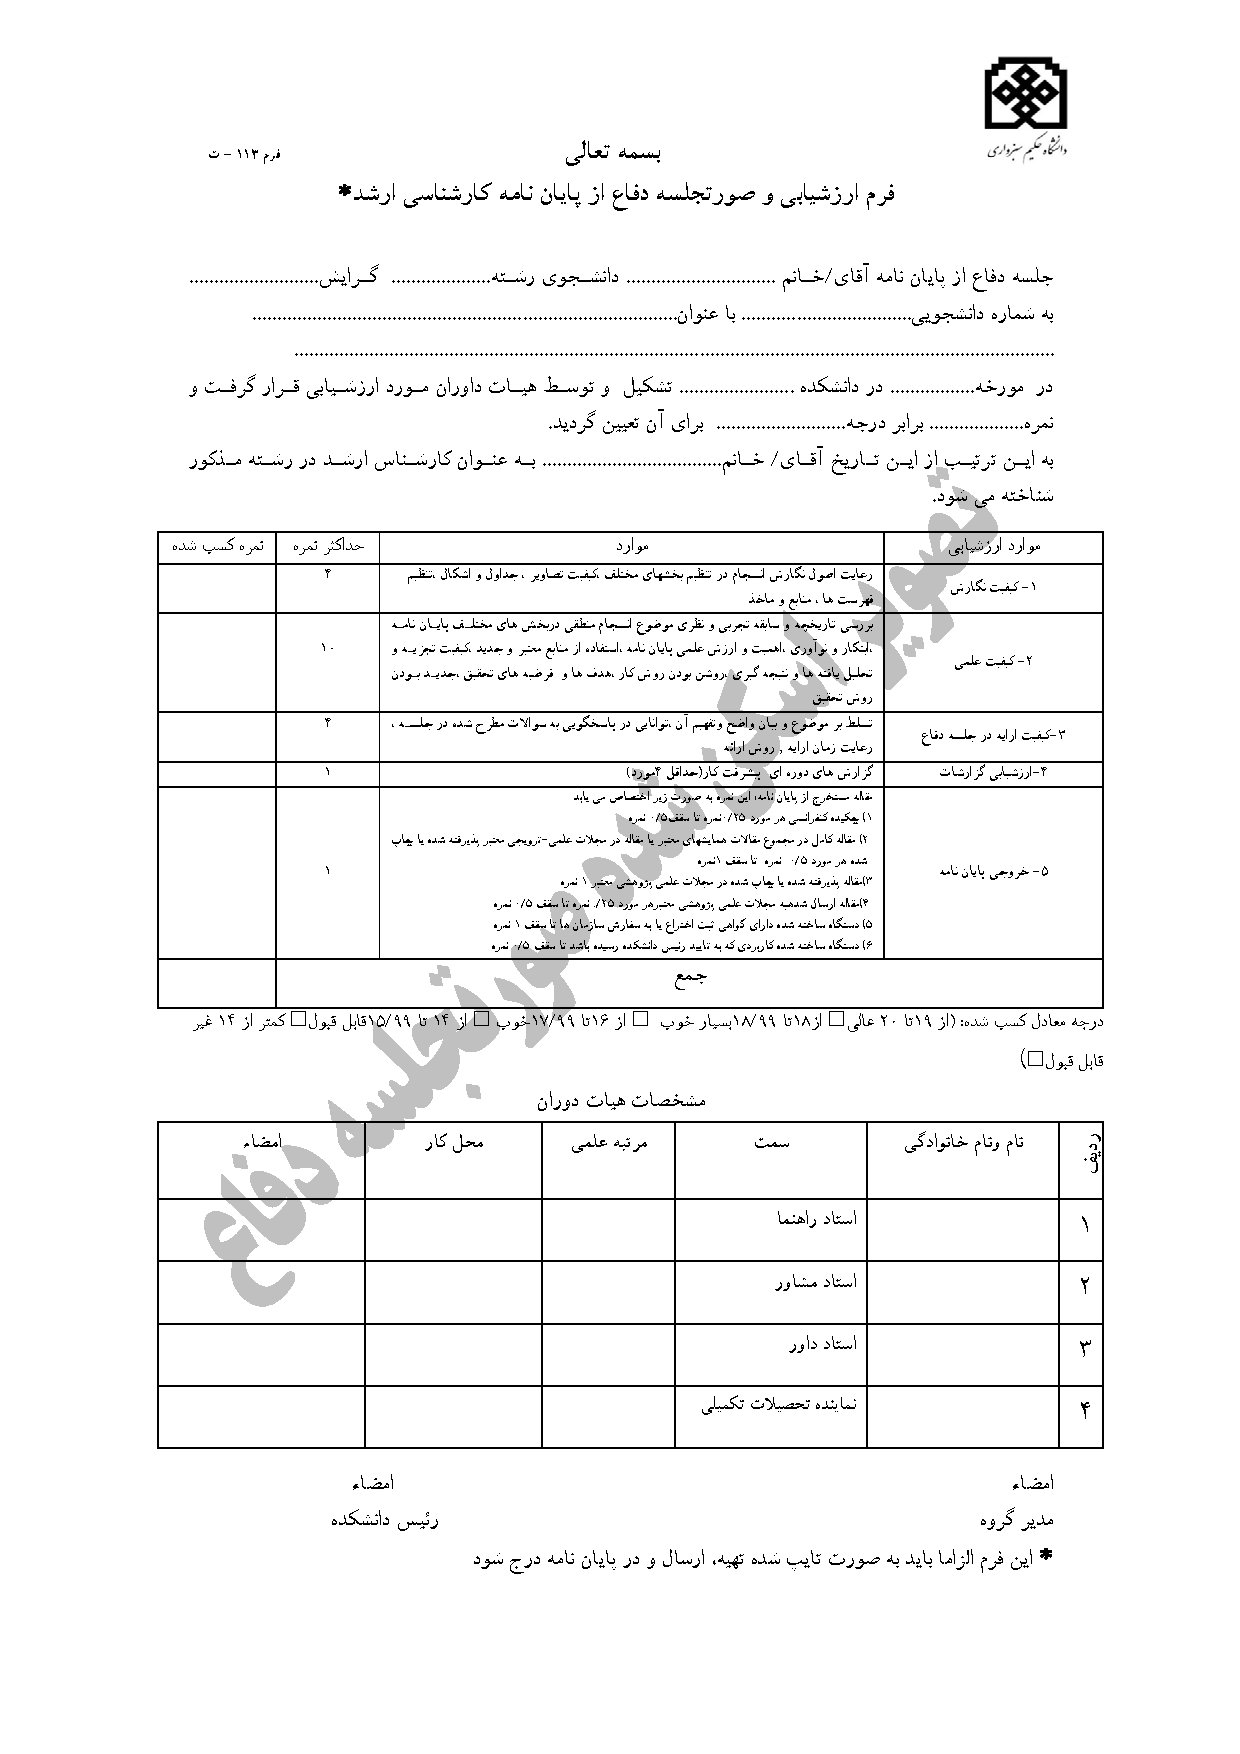
\includepdf{sooratjalaseh.pdf}!
در همان فایل را از حالت توضیح خارج کنید.
\end{enumerate}
دقت داشته باشید که اگر فایل اسکن شده شما، نامی به جز 
\lr{sooratjalaseh}
دارد یا باید نام آنرا به همین عبارت تغییر دهید و یا نام فایل خود را در  دستور فوق قرار دهید.
جدول اطلاعات داوران در فایل
\lr{davaranJadval.tex}
قرار دارد.

\subsection{مراجع}
برای وارد کردن مراجع \پ خود، کافی است فایل 
\lr{MyReferences.bib}
را باز کرده و مراجع خود را مانند مراجع داخل آن، وارد کنید.  سپس از \lr{bibtex} برای تولید مراجع با قالب مناسب استفاده کنید. برای توضیحات بیشتر بخش \ref{Sec:Ref} و پیوست
\eqref{App:App1} را ببینید.


\subsection{واژه‌نامه و نمایه}
برای وارد کردن واژه‌نامه فارسی به انگلیسی و برعکس، چنانچه کاربر مبتدی هستید، بهتر است مانند روش بکار رفته در فایل‌های 
\lr{dicfa2en}
و
\lr{dicen2fa}
عمل کنید. اما چنانچه کاربر پیشرفته هستید، بهتر است از بسته
\lr{glossaries}
استفاده کنید. 
برای وارد کردن نمایه، باید از 
\lr{xindy}
استفاده کنید. 
%زیرا 
%\lr{MakeIndex}
%با حروف «گ»، «چ»، «پ»، «ژ» و «ک» مشکل دارد و ترتیب الفبایی این حروف را رعایت نمی‌کند. همچنین، فاصله بین هر گروه از کلمات در 
%\lr{MakeIndex}،
%به درستی رعایت نمی‌شود که باعث زشت شدن حروف‌چینی این قسمت می‌شود. 
راهنمای چگونگی کار با 
\lr{glossaries} و \lr{xindy} 
را می‌توانید در
 \href{http://wiki.parsilatex.com}{ویکی پارسی‌لاتک} 
 مشاهده فرمایید.

\section{اگر سوالی داشتم، از کی بپرسم؟}
برای پرسیدن سوال های خود موقع حروف‌چینی با زی‌پرشین،  می‌توانید به
 \href{http://qa.parsilatex.com}{سایت پرسش و پاسخ پارسی‌لاتک}%
\LTRfootnote{\url{http://qa.parsilatex.com}}
مراجعه کنید. شما هم می‌توانید روزی به سوال های دیگران در این تالار، جواب بدهید.
بسته ی زی‌پرشین و بسیاری بسته‌های مرتبط با آن مانند \lr{bidi} و \lr{Persian-bib}، مجموعه پارسی‌لاتک، مثالهای مختلف موجود در آن و سایت پارسی‌لاتک همه به صورت داوطلبانه توسط افراد گروه 
\lr{Persian TeX}
و گروه پارسی‌لاتک و بدون هیچ کمک مالی انجام شده‌اند. کار اصلی نوشتن و توسعه زی‌پرشین توسط آقای وفا خلیقی انجام شده است که‌این کار بزرگ را به انجام رساندند.
اگر مایل به کمک به گروه پارسی‌لاتک هستید به سایت گروه پارسی‌لاتک مراجعه فرمایید:
%\begin{center}
 \href{http://www.parsilatex.com}{http://www.parsilatex.com} 
%\end{center}
    
\section{جمع بندی}
در این فصل به بیان مقدمات نحوه استفاده از قالب پایان‌نامه دانشگاه حکیم سبزواری پرداخته شد. گرچه که مطالعه کامل این راهنما مقداری وقت شما را خواهد گرفت، اما مطمئن باشید از اتلاف وقت شما در ادامه کارتان تا حد زیادی جلوگیری خواهد کرد. در نوشتن متن حاضر سعی شده است بیشتر مواردی که عموماً دانشجوان با آن مواجه هستند - و با نگاه ویژه به نیازهای دانشجویان ریاضی - ذکر شود. در ادامه نوشتار نمونه مواردی از درج تصویر، نمودار، کد برنامه، الگوریتم، توضیحات، منابع، فرمول، تعریف، قضیه، مثال و جدول آمده است. توصیه می‌شود یک کپی از کل فایلهای این قالب را جداگانه از نسخه \پ خود نگهداری نمایید تا در صورت نیاز بتوانید مراجعه فرمایید. همچنین توصیه اکید دارم که رفع خطاهایی که احتمالاً با آن مواجه می‌شوید را با آخر موکول نفرمایید و به محض برخورد با خطا، آنرا اشکال‌زدایی نموده و خطا را برطرف فرمایید.

